% ICISC format (LNCS / llncs.cls)
\documentclass[runningheads]{llncs}

\usepackage[T1]{fontenc}
\usepackage{graphicx}
\usepackage{url}
\usepackage{cryptocode}
\usepackage{algorithm}
\usepackage{algpseudocode}
\usepackage{amsmath}
\usepackage{enumitem}
\usepackage{amssymb}
\usepackage{subfig}
\usepackage{booktabs}
\usepackage{adjustbox}
\usepackage{multirow}
\usepackage{float}
\usepackage{pgfplots}
\pgfplotsset{compat=1.18}

% Color gradient definitions for multi-spec figures
% Fig 5: Red gradient (Naive) / Blue gradient (Freivalds)
\definecolor{redspec1}{RGB}{240, 140, 140}
\definecolor{redspec2}{RGB}{220, 90, 90}
\definecolor{redspec3}{RGB}{200, 50, 50}
\definecolor{redspec4}{RGB}{160, 20, 20}
\definecolor{redspec5}{RGB}{110, 0, 0}
\definecolor{bluespec1}{RGB}{120, 170, 240}
\definecolor{bluespec2}{RGB}{80, 130, 210}
\definecolor{bluespec3}{RGB}{50, 100, 190}
\definecolor{bluespec4}{RGB}{25, 60, 150}
\definecolor{bluespec5}{RGB}{0, 25, 100}
% Fig 6: Orange gradient (BERT) / Green gradient (Nystrom)
\definecolor{ornspec1}{RGB}{245, 170, 80}
\definecolor{ornspec2}{RGB}{230, 130, 40}
\definecolor{ornspec3}{RGB}{200, 100, 10}
\definecolor{ornspec4}{RGB}{170, 70, 0}
\definecolor{ornspec5}{RGB}{120, 45, 0}
\definecolor{grnspec1}{RGB}{100, 190, 120}
\definecolor{grnspec2}{RGB}{50, 160, 80}
\definecolor{grnspec3}{RGB}{20, 130, 50}
\definecolor{grnspec4}{RGB}{0, 100, 30}
\definecolor{grnspec5}{RGB}{0, 65, 15}

\newcommand{\name}{{\bf zkDietFormer}}
\newcommand{\scheme}{{\bf zkDiet}}
\newcommand{\Q}{{\mathbf{Q}}}
\newcommand{\K}{{\mathbf{K}}}
\newcommand{\V}{{\mathbf{V}}}
\newcommand{\W}{{\mathbf{W}}}
\newcommand{\sfmax}{{\mathrm{softmax}}}
\newcommand{\X}{{\mathbf{X}}}
\newcommand{\Y}{{\mathbf{Y}}}
\newcommand{\Z}{{\mathbf{Z}}}
\newcommand{\F}{{\mathbb{F}}}
\newcommand{\nystrom}{{\text{Nystr\"om }}}
\newcommand{\nystromformer}{{\text{Nystr\"omformer }}}
\newcommand{\rand}{{\mathbf{r}}}

% SNARK
\newcommand{\setup}{{\sf Setup}}
\newcommand{\prove}{{\sf Prove}}
\newcommand{\verify}{{\sf Verify}}
\newcommand{\pk}{{\sf pk}}
\newcommand{\vk}{{\sf vk}}
\newcommand{\ck}{{\sf ck}}
\newcommand{\crs}{{\sf crs}}
\newcommand{\td}{{\sf td}}
\newcommand{\sPi}{{\sf \Pi}}
\newcommand{\bPi}{{\bf \Pi}}
\newcommand{\ins}{{\mathbf{x}}}
\newcommand{\wit}{{\mathbf{w}}}
\newcommand{\comwit}{{\mathbf{u}}}
\newcommand{\uncomwit}{{\mathbf{\omega}}}
\newcommand{\cp}{{\sf cp}}
\newcommand{\cc}{{\sf cc}}


% Commitment
\newcommand{\Com}{{\sf Com}}
\newcommand{\cm}{{\sf cm}}
\newcommand{\commit}{{\sf Commit}}
\newcommand{\kzg}{{\sf KZG}}
\newcommand{\ped}{{\sf Ped}}
\newcommand{\gp}{{\sf gp}}
\newcommand{\comparams}{\textsf{CommitParams}}


% Nystromformer
\newcommand{\selectLandmarks}{{\sf SelectLandmarks}}
\newcommand{\computeMPInverse}{{\sf ComputeMPInverse}}
\newcommand{\NystromAttention}{\textsf{Nystr\"omAttention}}



%common
\newcommand{\R}{{\mathcal{R}}}
\newcommand{\A}{{\mathcal{A}}}
\newcommand{\E}{{\mathcal{E}}}
\newcommand{\sss}[1]{\noindent{\bf #1}.}
\newcommand{\ssi}[1]{\noindent{\it #1}.}
\newcommand{\sample}{{\overset{{\scriptscriptstyle\$}}{\leftarrow}}}

% Security
\newcommand{\negl}{{\sf negl}}

\newcommand{\krev}[1]{{\color{magenta}{#1}}}
\newcommand{\brev}[1]{{\color{blue}{#1}}}

\newcommand{\ckglob}{\mathsf{ck}_{\mathrm{glob}}}
\newcommand{\link}{\mathsf{link}}
\newcommand{\lkp}{\mathsf{lkp}}
\newcommand{\keygen}{\mathsf{KeyGen}}

\begin{document}

\title{\name: Verifiable Transformer Inference with Linear-Cost Attention Proofs via Low-Rank Approximation}
\titlerunning{zkDietFormer}

\author{First Author\inst{1} \and
Second Author\inst{2} \and
Third Author\inst{3}}

\authorrunning{F. Author et al.}

\institute{Institute 1 \and
Institute 2 \and
Institute 3}

\maketitle

\begin{abstract}
The widespread deployment of Transformer-based models via Model-as-a-Service platforms raises a fundamental trust problem: users cannot verify that the provider faithfully executed the claimed model on their input. Zero-knowledge SNARKs (zk-SNARKs) can bridge this gap by letting the provider prove correct inference without revealing proprietary model weights, yet existing approaches face an $O(n^2)$ proving-cost bottleneck rooted in the quadratic self-attention mechanism.
    
We propose $\name$, the first zero-knowledge verification framework designed for low-rank self-attention. By instantiating the Nystr\"{o}m approximation inside the proving circuit, we replace the full $n \times n$ attention computation, including the nonlinear cost induced by the row-wise softmax, with three smaller matrix products involving only $m \ll n$ landmark tokens, reducing the dominant cost to $O(n)$. The pseudoinverse factor is supplied as a witness and constrained in-circuit via the Moore--Penrose conditions, avoiding its explicit computation. We further verify large matrix products through Freivalds' single random-vector checks, and employ commit-carrying SNARKs that offload weight commitments outside the circuit while binding every response to a single committed model.
    
Experiments on five BERT-scale configurations (hidden dimensions 128--768, depths 2--12) show that zkDietFormer extends the maximum provable sequence length by up to $4\times$ over standard attention under the same 128\,GB memory budget, with per-layer prove time growing near-linearly in $n$. Under 26-bit fixed-point arithmetic, the quantized model preserves 98.8\% top-1 agreement with its floating-point counterpart.
    
\keywords{Zero-Knowledge Proofs \and Verifiable AI \and Low-Rank Attention \and Transformer \and zk-SNARKs}
\end{abstract}

%-------------------------------------------------------------------------------
\section{Introduction}
%-------------------------------------------------------------------------------
Recent breakthroughs in Transformer-based models have revolutionized artificial intelligence, facilitating the widespread deployment of high-performance Large Language Models (LLMs) via Model-as-a-Service (MaaS) platforms. In this setting, model providers typically large models, while users receive outputs through APIs or remote inference interfaces. However, this architecture inherently obscures the generation process: users cannot independently verify whether the received output truly produced from the specific model architecture and weight parameters intended. Users are therefore forced to rely on trust regarding whether the provider substituted a cheaper model for the same input, post-processed or modified outputs due to internal policies, or unintentionally changed the model during updates or deployment. This problem of model execution integrity is particularly critical in high-stakes domains such as finance, healthcare, and security, and becomes increasingly central as demands for transparency and accountability in inference continue to grow.

One may attempt to address this trust issue by requiring the model provider to disclose model parameters for verification. In practice, however, this is practically infeasible. Model weights are the result of substantial investments in data, compute, and engineering, and are protected as proprietary intellectual property (IP). Consequently, a fundamental dilemma arises: users demand integrity guarantees for the model's outputs, while providers must preserve the privacy of their model parameters to protect their assets.

Zero-knowledge proofs (ZKPs) provide a principled way to reconcile these conflicting requirements. By leveraging ZKPs, a prover (the model provider) can cryptographically prove that an output $y$ is the result of evaluating the model on the user's input $x$ with a secret weight $W$, i.e., $f(x, W) = y$, without revealing any information about $W$ itself. This enables verifiable inference while maintaining the confidentiality of model parameters.

However, making ZKP-based verifiable AI practically deployable requires the efficient proving of computationally intensive deep learning operations. In modern Transformer architectures, the primary bottleneck is the self-attention mechanism, the computational core of the model. For an input sequence of length $n$ and hidden dimension $d$, the input $X \in \mathbb{R}^{n \times d}$ is projected into queries, keys, and values $\Q, \K, \V \in \mathbb{R}^{n \times d}$ (for a single attention head). Standard self-attention forms an attention matrix $\Q\K^\top \in \mathbb{R}^{n\times n}$, applies a row-wise softmax over the entire matrix, and then multiplies by $\V$ to obtain the attention output.

This computation requires $\mathcal{O}(n^2d)$ linear operations for matrix multiplications, as well as an additional $\mathcal{O}(n^2)$ nonlinear cost induced by the softmax. The resulting computational overhead is substantial, posing the single largest obstacle to proving large-scale Transformer models.

The most na\"ive approach to proving self-attention involves arithmetizing the full $\Q\K^\top$ computation into a circuit and enforcing the resulting $\mathcal{O}(n^2 d)$ operations within a SNARK. However, this cost far exceeds practical limits. To mitigate this, many systems have adopted probabilistic verification techniques for large matrix products, such as Freivalds' algorithm~\cite{Freivalds} or Thaler's randomized checks~\cite{Thaler}. These methods verify the $n \times n$ multiplication relation without full recomputation by sampling random vectors, compressing verification to a small number of checks and reducing the cost to $\mathcal{O}(n^2)$. Nevertheless, the complexity remains dominated by the quadratic term, which becomes increasingly prohibitive as models scale. For instance, while BERT~\cite{BERT} uses 512 tokens and GPT-3~\cite{GPT3} uses a 2,048-token context window, frontier models now support contexts in the hundreds of thousands or even millions (e.g., 400K for GPT-5~\cite{GPT5} and 10M for Llama~4 Scout~\cite{llama4}). As $n$ grows, this quadratic verification cost renders proof generation for realistic sequence lengths impractical.

Meanwhile, deep learning literature has repeatedly demonstrated that attention matrices often exhibit an approximate low-rank structure. Concretely, when the number of landmarks $m \ll n$, the attention matrix can be effectively approximated by a rank-$m$ representation, enabling training and inference costs to approach linearity with respect to the sequence length~\cite{Linformer,Nystromformer}. Despite these advances, the field of Verifiable AI has yet to exploit low-rank structures as a primary mechanism for reducing proof generation costs. Consequently, a gap persists: while low-rank approximations improve computational efficiency in practice, the lack of proof systems tailored to these structures keeps proof complexity anchored at $\mathcal{O}(n^2)$. This work aims to bridge this gap. Our central idea is to combine low-rank structures with probabilistic verification to eliminate the quadratic complexity in verifying self-attention matrices.

\subsection{Our Contribution}
In this work, we propose \name, a verification protocol that eliminates the dominant $\mathcal{O}(n^2)$ bottleneck in proving self-attention by combining a low-rank representation of the attention matrix, Freivalds' randomized checks, and a commit-carrying SNARK. Our main contributions are summarized as follows:
\begin{itemize}
    \item \textbf{The first verification framework tailored to low-rank self-attention.} To the best of our knowledge, we present the first verification framework specifically designed for low-rank self-attention. We instantiate this framework using the \nystrom method, reducing the overall circuit complexity---including both the core matrix operations of self-attention and the nonlinear operations induced by row-wise softmax---to $\mathcal{O}(n)$.
    \item \textbf{Constraint-efficient verification via Freivalds' checks and CC-SNARKs.} We employ Freivalds' algorithm to efficiently verify large matrix computations inside the circuit, while leveraging commit-carrying SNARKs to offload computationally expensive operations outside the circuit, significantly reducing the total number of constraints.
    \item \textbf{Practical implementation and evaluation.} We implemented a prototype of the proposed framework and evaluated its performance through benchmarks. The results demonstrate a significant reduction in prover costs for practical sequence lengths, showing that \name is not only theoretically efficient but also practically deployable.
\end{itemize}

In summary, the prover's constraint cost in \name scales linearly with the input sequence length $n$. Consequently, to the best of our knowledge, this work provides the first verifiable mechanism for low-rank self-attention that enables proof generation with cost linear to the sequence length.



%-------------------------------------------------------------------------------
\section{Related Works}\label{sec:related}

\textbf{Low-Rank Transformer.}
Standard Transformer attention~\cite{OriginalTransformer} has $O(n^2)$ complexity. Sparse patterns~\cite{SparseTransformer,Longformer} and memory compression~\cite{CompressiveTransformer} reduce cost but sacrifice full attention. Low-rank methods restore linear complexity while preserving the full attention structure: Linformer~\cite{Linformer} projects keys and values into a lower-dimensional space; Performer~\cite{Performer} approximates softmax via random-feature kernelization; and Nystr\"omformer~\cite{Nystromformer} reconstructs the attention map from $m$ landmark tokens via the Nystr\"om method, achieving higher accuracy than Performer with $O(n)$ complexity.

\textbf{zk-SNARKs for Matrix Multiplication.}
Thaler~\cite{Thaler} reduces matrix-multiplication verification to $O(n^2)$ via Sumcheck; zkCNN~\cite{zkCNN} and zkML~\cite{zkML} adopt this for neural-network layers, the latter using Freivalds' algorithm~\cite{Freivalds}. pvCNN~\cite{pvCNN} and vCNN~\cite{vCNN} cast convolution as a single matrix product verified through Quadratic Matrix Programs. zkLLM~\cite{zkLLM} achieves prover complexity linear in tensor size via specialized sumcheck protocols, building on SafetyNets~\cite{SafetyNets}. zkMatrix~\cite{zkMatrix} uses Bulletproofs-based acceleration for $O(n^2)$ prover time with $O(\log n)$ verification. However, all these approaches retain $O(n^2)$ prover cost in the matrix dimension~\cite{Thaler,zkCNN,vCNN,zkML,zkMatrix} or face prohibitively large auxiliary dimensions~\cite{zkLLM}, and nonlinear functions such as softmax require approximation~\cite{zkVC}.

%-------------------------------------------------------------------------------
\section{Preliminaries}
\label{sec:preliminaries}
%-------------------------------------------------------------------------------

\sss{Notation}
We denote the sequence length by $n$, the hidden dimension by $d$, and the per-head query/key and value dimensions by $d_k$ and $d_v$, respectively. The number of attention heads is $h$, the number of Transformer layers is $L$, and the number of landmarks is $m$, giving a segment length $\ell = n/m$. The circuit precision parameter $k_{\text{bits}}$ controls the bit-width of quantized fixed-point arithmetic.

\subsection{Scaled Dot-Product Attention}
The model represents interactions between tokens using queries and keys of dimension $d_k$, and values of dimension $d_v$. For each token, its associated query computes its similarity scores with the keys of all other tokens in the sequence, thereby determining which parts of the input the model should attend to more strongly. The contextual information is then aggregated by computing a weighted sum of the corresponding value vectors based on these similarities.

The attention mechanism is defined as a function that takes a single query together with a set of key--value pairs and produces an output vector, where the query, keys, values, and outputs all lie in vector spaces. In practice, multiple queries are processed simultaneously by stacking them into matrices $\Q$, $\K$, and $\V$. These matrices are obtained by projecting the input matrix $\X \in \mathbb{R}^{n \times d}$ using learnable parameter matrices $\W^Q \in \mathbb{R}^{d \times d_k}$, $\W^K \in \mathbb{R}^{d \times d_k}$, and $\W^V \in \mathbb{R}^{d \times d_v}$, yielding $\Q = \X \W^Q \in \mathbb{R}^{n \times d_k}$, $\K = \X \W^K \in \mathbb{R}^{n \times d_k}$, and $\V = \X \W^V \in \mathbb{R}^{n \times d_v}$. Concretely, the attention weights are obtained by scaling the dot product between queries and keys by $1/\sqrt{d_k}$, followed by the application of the softmax function. The final output is computed as the weighted sum of the value vectors using these attention weights.

The output matrix is computed as follows:
\[
    \text{Attention} (\Q, \K, \V ) = \sfmax\left(\frac{\Q\K^\top}{\sqrt{d_k}}\right)\V
\]


\subsection{Multihead Attention}
Multi-head attention replaces a single attention function over $d$-dimensional queries, keys, and values with $h$ parallel attention heads. The queries, keys, and values are first linearly projected $h$ times into lower-dimensional subspaces of sizes $d_k$ and $d_v$, respectively. For each head $i$,
\[
    \text{head}_i = \text{Attention} (\Q_i, \K_i, \V_i)
\]
where $\Q_i = \X \mathbf{W}_i^{Q}$, $\K_i = \X \mathbf{W}_i^{K}$, $\V_i = \X \mathbf{W}_i^{V}$, with learnable projection matrices $\mathbf{W}_i^{Q} \in \mathbb{R}^{d\times d_k}, \mathbf{W}_i^{K} \in \mathbb{R}^{d\times d_k}$, and $\mathbf{W}_i^{V} \in \mathbb{R}^{d\times d_v}$.
The resulting head outputs are concatenated and linearly transformed to form the final representation:
\[
\text{MultiHead}(\Q,\K,\V)=\text{Concat} (\text{head}_1,\dots,\text{head}_h) \mathbf{W}^{O}
\]
with $\mathbf{W}^{O} \in \mathbb{R}^{h d_v \times d}$.
In the standard setting, $d_k = d_v = d/h$, so that the total cost across heads matches that of single-head attention over $d$ dimensions. This design enables the model to attend to diverse representation subspaces while maintaining computational cost comparable to single-head attention. For clarity, we describe the protocol for a single attention head with $d_k = d_v = d$; the extension to $h$ heads follows by applying the same construction per head.

\subsection{Nystrom-Based Linear Attention}\label{subsec:nystrom-linear}
Nystr\"omformer applies the Nystr\"om method~\cite{Nystromformer}---a technique widely used in matrix approximation---to reduce the computational complexity of the standard Transformer from $O(n^2)$ to $O(n)$. The key idea of the Nystr\"om method is to reconstruct the full matrix approximately by using only a subset of its rows and columns, instead of computing the entire matrix explicitly.

When the softmax matrix $S$ is expressed as a block matrix as shown below,
\[
    S = \sfmax(\frac{\Q\K^\top}{\sqrt{d_k}}) = \begin{bmatrix} A_S\ B_S \\ F_S\ C_S \end{bmatrix}
\]
the Nystrom method approximates the expensive block $C_S \in \mathbb{R}^{(n-m)\times (n-m)}$ by using the smaller blocks $A_S \in \mathbb{R}^{m \times m}, B_S \in \mathbb{R}^{m \times (n-m)}, F_S \in \mathbb{R}^{(n-m)\times m}$ as illustrated below:
\[
    \hat S = \begin{bmatrix}
            A_S & B_S \\
            F_S & F_S A_S^{+} B_S
            \end{bmatrix} =
            \begin{bmatrix}
            A_S \\
            F_S
            \end{bmatrix}
            A_S^{+}
            \begin{bmatrix}
            A_S & B_S
            \end{bmatrix}
\]
Here, $A_S^+$ denotes the Moore-Penrose pseudoinverse of $A_S$.

However, when this approach is applied directly to self-attention, the row-wise normalization property of the softmax function still requires accessing all entries of the $n \times n$ matrix in order to compute the denominators. To address this issue, Nystr\"omformer partitions the entire sequence into $m$ segments of length $\ell = n/m$ before applying softmax, and computes the mean within each segment to obtain $m$ landmark points for the queries and keys, respectively. These landmarks yield $\widetilde{\Q}, \widetilde{\K} \in \mathbb{R}^{m \times d}$, from which three low-rank factors $\Q\widetilde{\K}^\top \in \mathbb{R}^{n \times m}$, $\widetilde{\Q}\widetilde{\K}^\top \in \mathbb{R}^{m \times m}$, and $\widetilde{\Q}\K^\top \in \mathbb{R}^{m \times n}$ are formed. The resulting factors play the same structural role as $\begin{pmatrix} A_S \\ F_S \end{pmatrix}$, $A_S^{+}$, and $\begin{pmatrix} A_S & B_S \end{pmatrix}$ in the block decomposition above, but are computed from landmarks rather than extracted from~$S$.
Using these matrices, Nystr\"omformer derives a final approximation that achieves linear computational complexity:

\begin{align*}
\hat S V &=
\sfmax\!\left(\frac{\Q\widetilde{\K}^{\top}}{\sqrt{d_k}}\right)
\,
\sfmax\!\left(\frac{\widetilde{\Q}\widetilde{\K}^{\top}}{\sqrt{d_k}}\right)^{+}
\,
\sfmax\!\left(\frac{\widetilde{\Q}\K^{\top}}{\sqrt{d_k}}\right)V
\end{align*}

The exact computation of the pseudoinverse $A_S^{+}$ (e.g., via SVD) is computationally expensive and poorly suited for GPU execution, becoming a practical bottleneck in implementation. To mitigate this issue, Nystr\"omformer introduces an iterative algorithm that approximates the pseudoinverse using repeated matrix multiplications. The resulting approximation $Z^*$ is then substituted into the final formulation, significantly improving computational efficiency.

\begin{align*}
\hat S V &= \sfmax\!\left(\frac{\Q\widetilde{\K}^{\top}}{\sqrt{d_k}}\right)\, Z^* \,
\sfmax\!\left(\frac{\widetilde{\Q}\K^{\top}}{\sqrt{d_k}}\right)V
\end{align*}

\subsection{zk-SNARKs}
A \textit{zero-knowledge succinct non-interactive argument of knowledge} (zk-SNARK) for an NP relation $\R$ consists of three PPT algorithms $\Pi=(\setup,\prove,\verify)$: $(\pk,\vk)\gets\Pi.\setup(1^\lambda,\R)$ outputs a proving key and verification key; $\pi\gets\Pi.\prove(\pk,\ins;\wit)$ produces a proof for statement $\ins$ and witness $\wit$ with $(\ins,\wit)\in\R$; and $0/1\gets\Pi.\verify(\vk,\ins,\pi)$ accepts or rejects. A zk-SNARK satisfies \emph{completeness} (an honest prover always convinces the verifier), \emph{knowledge soundness} (an accepting proof implies the prover knows a valid witness), \emph{zero-knowledge} (the proof reveals nothing beyond the statement's truth), and \emph{succinctness} (the proof size is $|\pi|=\mathit{poly}(\lambda)\cdot\mathit{polylog}(|\ins|+|\wit|)$). Formal definitions appear in~\cite{Groth16}.

\sss{Commit-and-Prove SNARKs (CP-SNARKs)}
CP-SNARKs~\cite{Legosnark,Lunar} let a prover demonstrate that values hidden inside a commitment $\cm=\Com(\comwit;o)$ satisfy a relation $\R$. The witness is split as $\wit:=(\uncomwit,\comwit,o)$, where $\comwit$ is committed and $\uncomwit$ is not. The interface mirrors a plain SNARK except that Setup additionally takes a commitment key $\ck$, Prove takes $\cm$ as part of the statement and includes $(\comwit,o)$ in the witness, and Verify checks both the relation and the commitment consistency.

\sss{Commit-Carrying SNARKs (CC-SNARKs)}
CC-SNARKs~\cite{Legosnark,Vectis} extend CP-SNARKs by generating the commitment \emph{during} proving rather than beforehand. The setup outputs a circuit-dependent commitment key $\ck$ alongside $(\pk,\vk)$. The prover partitions the witness as $\wit:=(\comwit,\uncomwit)$ and outputs both a proof $\pi_\cc$ and a commitment $\tilde{\cm}=\Com.\commit(\ck,\comwit;\tilde{o})$. The verifier checks $\Pi_\cc.\verify(\vk,\ins,\tilde{\cm},\pi_\cc)$. This design moves expensive group exponentiations outside the circuit, which is critical for scaling to large Transformer weight matrices.


\subsection{Freivalds' Algorithm}
Freivalds' algorithm~\cite{Freivalds,Korec} is a simple yet powerful randomized method for verifying a matrix product without recomputing it.
Let \(\X,\Y,\Z\in \mathbb{F}^{n\times n}\) and consider the claim \(\X \cdot \Y=\Z\).
Instead of computing \(\X\Y\) in \(\mathcal{O}(n^3)\) time, Freivalds samples a uniformly random vector \(\mathbf{r}\sample \mathbb{F}^n\) and checks
\[
\X(\Y\mathbf{r}) \stackrel{?}{=} \Z\mathbf{r}.
\]
This verification runs in \(\mathcal{O}(n^2)\) field operations. This algorithm has soundness error: if \(\X\Y=\Z\), it always accepts.
Otherwise, when \(\X\Y\neq \Z\), the check passes with probability at most \(1/|\mathbb{F}|\), i.e.,
\[
\Pr\!\big[\,\X(\Y\mathbf{r}) = \Z\mathbf{r}\ \big|\ \X\Y\neq \Z\,\big] \le \frac{1}{|\mathbb{F}|}.
\]
The same principle extends to rectangular matrices and to the transposed (left-multiplied) variant $\mathbf{r}^{\top}\!\X\Y \stackrel{?}{=} \mathbf{r}^{\top}\!\Z$, which we use in Section~\ref{sec:protocol} to verify products of varying dimensions.

%-------------------------------------------------------------------------------
\section{Technical Overview}
\label{sec:overview}
%-------------------------------------------------------------------------------

Among the low-rank attention mechanisms reviewed in Section~\ref{sec:related}, we adopt Nystr\"omformer~\cite{Nystromformer} because it requires no additional learned projection matrices in the proving circuit and provides numerically stable reconstruction regardless of sequence length. We exclude Performer~\cite{Performer}, whose FAVOR+ random feature map introduces nonlinear exponential evaluations that would increase circuit complexity.

\begin{figure}[!ht]
    \centering
    \subfloat[Nystr\"omformer matrix approximation\label{fig:nystrom-approx}]{%
        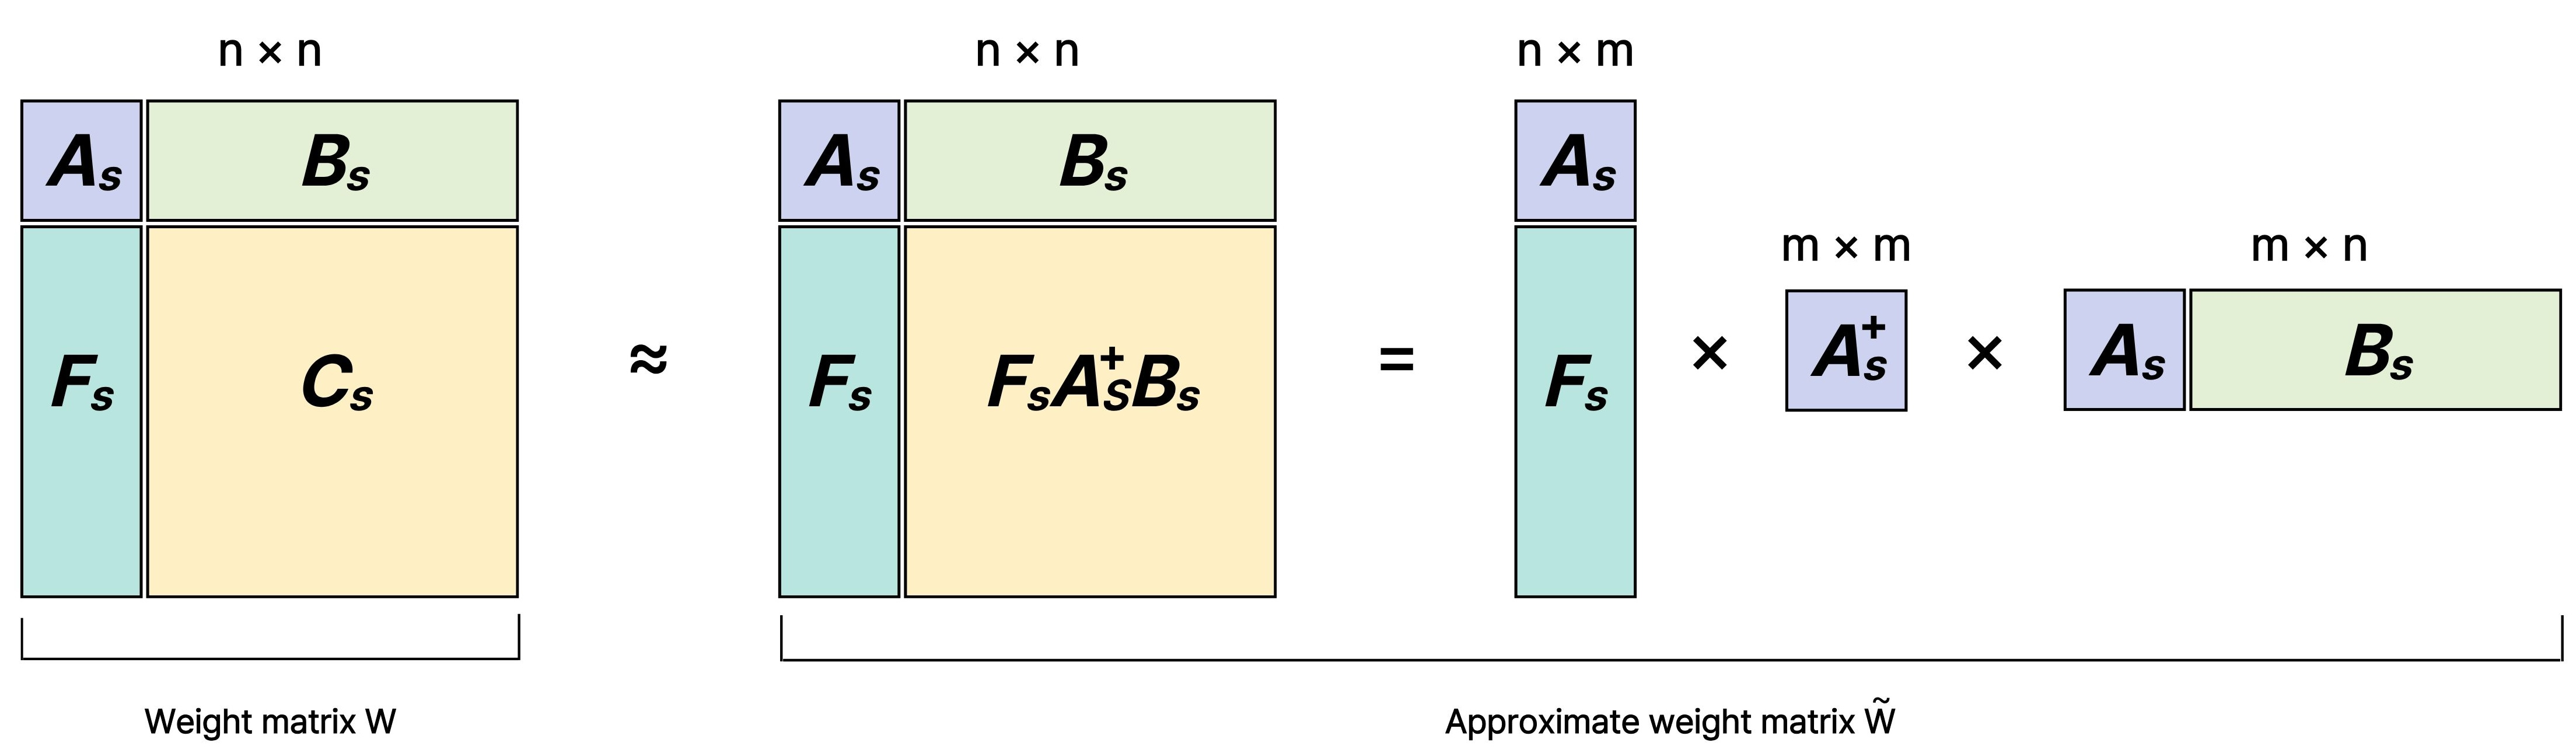
\includegraphics[width=\textwidth]{../images/nystrom-approx.jpg}%
    }\\[6pt]
    \subfloat[Our \name{} Freivalds' Check\label{fig:zkdiet}]{%
        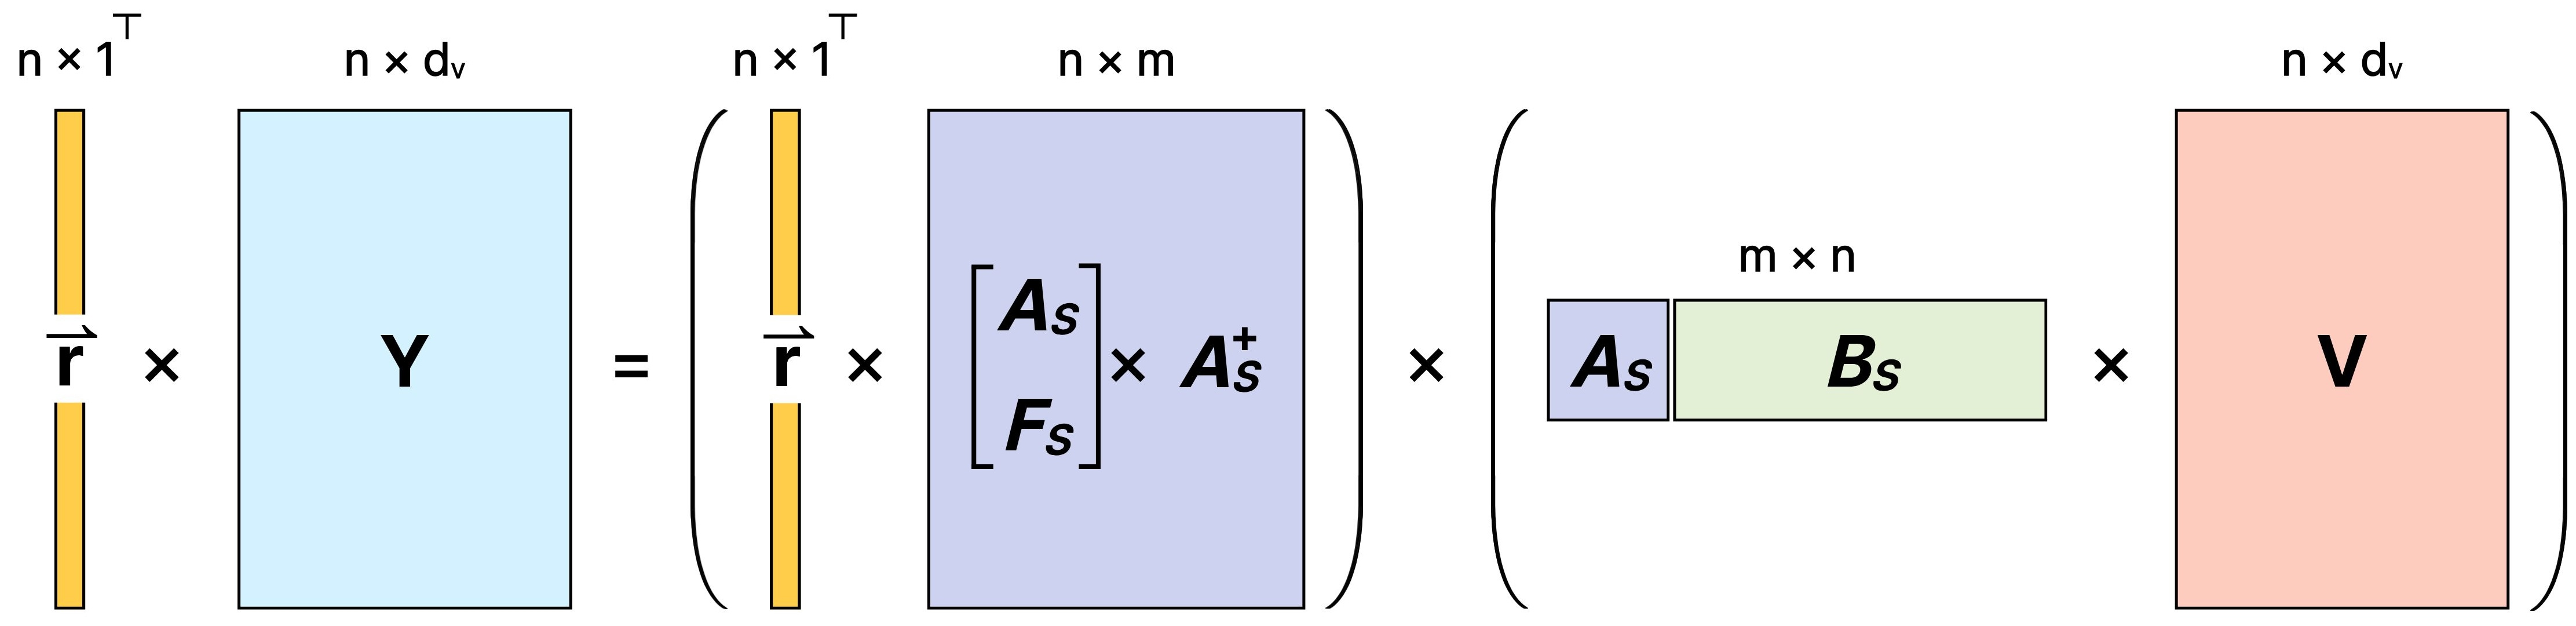
\includegraphics[width=\textwidth]{../images/zkdiet-freivald.jpg}%
    }
    \caption{Low-rank matrix multiplication with Freivalds' algorithm}
\end{figure}

As illustrated in Figure~\ref{fig:nystrom-approx}, rather than directly handling the $n \times n$ self-attention matrix, we follow the Nystr\"omformer procedure and decompose it into a sequence of low-dimensional matrices of shapes $n \times m$, $m \times m$, and $m \times n$. we denote the three low-rank factors by
$\tilde{F} := \mathrm{softmax}(Q\tilde{K}^{\top}/\sqrt{d_k}) \in \mathbb{F}^{n \times m}$,
$\tilde{A} := \mathrm{softmax}(\tilde{Q}\tilde{K}^{\top}/\sqrt{d_k}) \in \mathbb{F}^{m \times m}$, and
$\tilde{B} := \mathrm{softmax}(\tilde{Q}K^{\top}/\sqrt{d_k}) \in \mathbb{F}^{m \times n}$,
treated formally in Section~\ref{subsec:nystrom-attention}.
In the block decomposition of Figure~\ref{fig:nystrom-approx}, $\tilde{F}$, $\tilde{A}^{+}$, and
$\tilde{B}$ take the roles of
$\bigl[\begin{smallmatrix} A_S \\ F_S \end{smallmatrix}\bigr]$,
$A_S^{+}$, and $\bigl[\, A_S \;\; B_S \,\bigr]$, respectively;
they are computed from the landmarks before the softmax rather than
extracted from $S$ (cf.\ Section~\ref{subsec:nystrom-linear}), so Figure~\ref{fig:zkdiet} is obtained from
Figure~\ref{fig:nystrom-approx} by this substitution. By applying Freivalds' algorithm to this low-rank representation (Figure~\ref{fig:zkdiet}), we compress the verification workload from $O(n^2)$ to $O(n)$, effectively reducing it to a chain of vector--matrix products of total size $2nm + m^2 + nd_v$: multiplying the random vector by $\tilde{F}$ ($nm$), then by $\tilde{A}^{+}$ ($m^2$), then by $\tilde{B}$ ($mn$), and finally by~$\V$ ($nd_v$). The pseudoinverse factor is instantiated by the iterative approximation $Z^{*}$ of Section~\ref{subsec:nystrom-linear}: the prover computes $Z^{*}$ outside the circuit and supplies it as a witness, and our protocol verifies in-circuit that $Z^{*}$ satisfies the Moore--Penrose conditions (Section~\ref{moore-penrose}) up to quantization tolerance. Since these conditions uniquely characterize the pseudoinverse $\tilde{A}^{+}$, this check constrains $Z^{*}$ to a small neighborhood of $\tilde{A}^{+}$, without ever computing $\tilde{A}^{+}$ itself.

\begin{figure}[!ht]
    \centering
    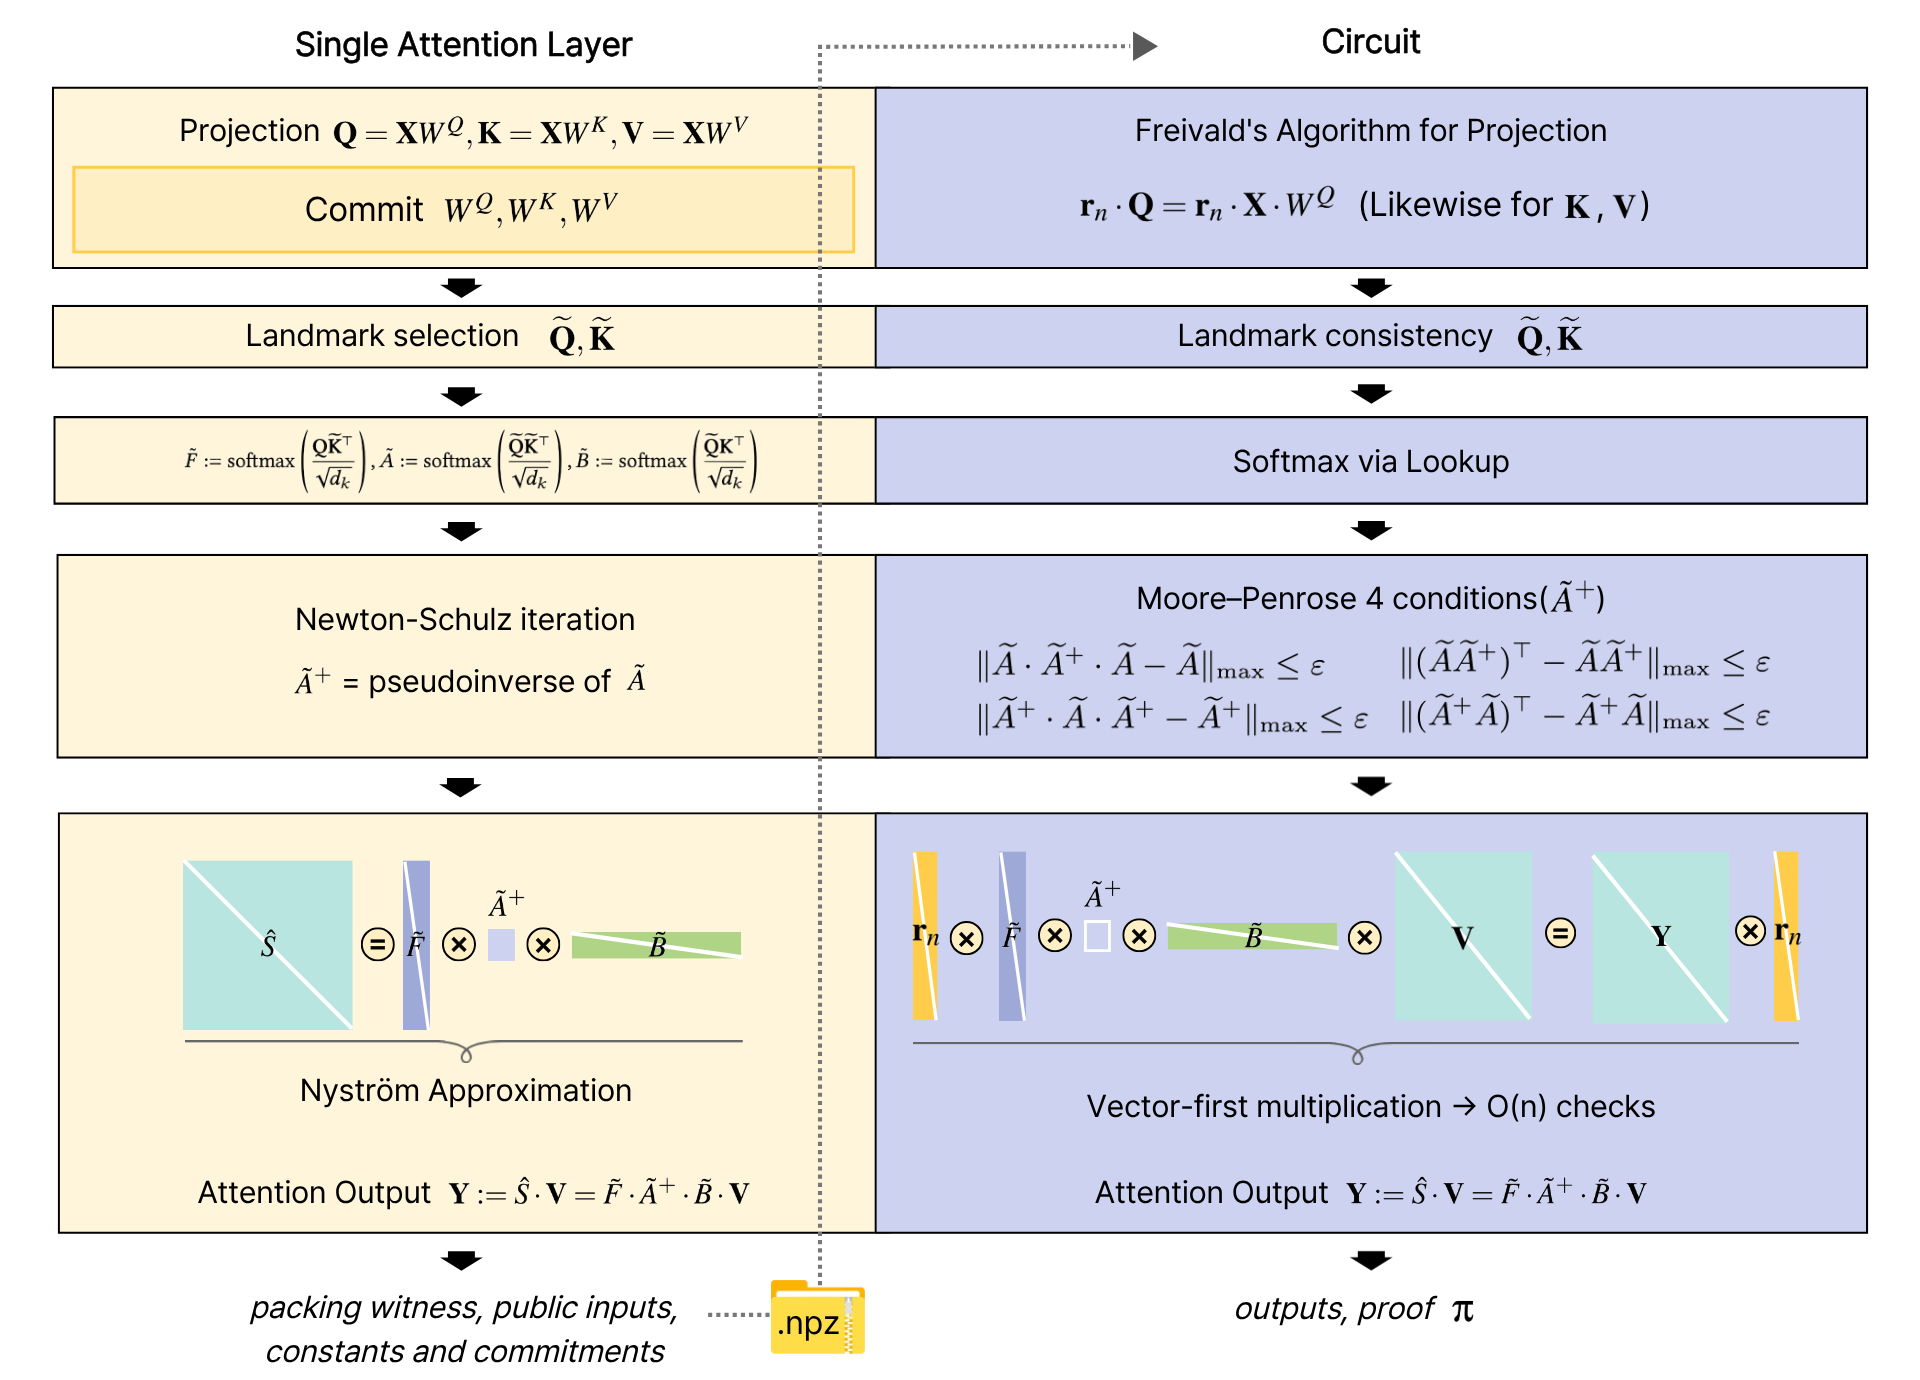
\includegraphics[width=\textwidth]{../images/overview.png}
    \caption{Overview of Self-Attention and our framework}
    \label{fig:attention-overview}
\end{figure}

We embed these low-rank checks in a commit-carrying SNARK (CC-SNARK) architecture (Figure~\ref{fig:attention-overview}): model weights are committed once under a circuit-independent key, and each proof carries a circuit-dependent commitment linked to the global one via CP-linkage, so the verifier needs only constant-time commitment checks (details in Section~\ref{sec:protocol}).
Because zero-knowledge circuits operate over finite fields, real-valued Transformer computations cannot be represented directly. We therefore quantize the computations in a manner that minimizes precision loss, leveraging the R1CS-friendly quantization technique proposed in~\cite{ZEN}. From this point onward, all matrices are understood to be over the finite field $\mathbb{F}$ after quantization.

\begin{figure}[!ht]
\centering
\newsavebox{\protocolbox}
\savebox{\protocolbox}{%
\fbox{\procedure[head=\textbf{Protocol}, bodylinesep=2mm]{}{
        \mathcal{P}(\ck, c_W, \X; \{ W^Q, W^K, W^V, W^O\}) \< \< \mathcal{V}(\vk, c_W, \X) \\
        (\Y', \textit{aux}, \mathsf{lk}) \gets \NystromAttention(\X, W^Q, W^K, W^V, W^O) \\
        \widetilde{\cm}_{W^i} \gets \Com.\commit(\ck,W^i;\tilde{o}_i) \text{ for } i \in \{Q,K,V,O\} \\
        \widetilde{\cm} \gets \Com.\commit(\ck, \mathsf{lk} ;\tilde{o}) \\
        \<  \sendmessageright*[2cm]{\{\widetilde{\cm}_{W^i}\}_{i \in \{Q,K,V,O\}}, \widetilde{\cm}, \Y'\;} \< \\
        \< \sendmessageleft*[2cm]{\rand_n, \rand_m } \< \rand_n \sample \F^n, \t \rand_m \sample \F^m  \\
        \ins := \{ \X, \Y', \rand_n, \rand_m \} \\
        \comwit := \{ (W^i,\tilde{o}_i)_{i \in \{Q,K,V,O\}}, (\mathsf{lk}, \tilde{o}), (W^i,o_i)_{i \in \{Q,K,V,O\}} \} \\
        \uncomwit := \textit{aux} \\
        \pi \gets \Pi_\mathsf{zkdiet}.\prove( \pk, \ins; (\comwit, \uncomwit)) \\
        \<  \sendmessageright*[2cm]\pi \< \\
        \< \< \Pi_\mathsf{zkdiet}.\verify(\vk, \ins, \{\widetilde{\cm}_{W^i}\}_{i \in \{Q,K,V,O\}},\, \widetilde{\cm}, c_W, \pi)
    }}%
}%
\resizebox{\columnwidth}{!}{\usebox{\protocolbox}}
    \caption{Our protocol}
    \label{fig:protocol}
\end{figure}

%-------------------------------------------------------------------------------
\section{\name: Efficient Proofs of Low-Rank Matrix Multiplication via Freivalds' Algorithm}
\label{sec:protocol}
%-------------------------------------------------------------------------------

In this section, we present the core protocol of \name. Our goal is to prove the correctness of \nystrom-approximated low-rank self-attention while avoiding any explicit computation of the $n \times n$ attention matrix inside the circuit. Concretely, we design the protocol so that the number of constraints scales linearly with the sequence length $n$. To this end, we adopt a commit-carrying SNARK (CC-SNARK) architecture that pushes computationally expensive operations (e.g., large matrix multiplications and pseudoinverse computation) outside the circuit, and proves only their correctness inside the circuit using a small number of constraints.


\subsection{Protocol Overview}
Our protocol follows the message flow of Figure~\ref{fig:protocol}. Prior to serving any query, the provider publishes a global commitment $c_W \gets \Com.\commit(\ck_{\mathrm{glob}}, W; o)$ to its weights $W=(W^Q,W^K,W^V,W^O)$ under a circuit-independent key $\ck_{\mathrm{glob}}$.

For each query with input $\X\in\mathbb{F}^{n\times d}$, the prover executes $\NystromAttention$ locally to obtain $\Y'$, non-linear operands $\mathsf{lk}:=(\tilde{F},\tilde{A},\tilde{B})$, and auxiliary intermediates $\textit{aux}$. It then commits to the weights and operands under the circuit-dependent key $\ck$, producing $\widetilde{\cm}_{W^i}$ and $\widetilde{\cm}$, and sends these commitments together with $\Y'$ to the verifier. The verifier replies with random challenges $\rand_n\sample\mathbb{F}^n$, $\rand_m\sample\mathbb{F}^m$.

The public instance is $\ins:=(\X,\Y',\rand_n,\rand_m)$. The committed witness $\comwit$ contains the weight matrices and their opening randomness (for both the global and circuit-dependent commitments) plus the non-linear operands; the uncommitted witness $\uncomwit:=\textit{aux}$ contains the remaining intermediates, each constrained by the chain of Freivalds checks linking committed weights to the public output $\Y'$. All commitments are fixed before challenges are sampled, preserving Freivalds soundness.

The prover generates a composite proof $\pi$ that encapsulates the CC-SNARK proof together with two CP-linkages binding the circuit-dependent commitments $\{\widetilde{\cm}_{W^i}\}$ to the global $c_W$ and $\widetilde{\cm}$ to the lookup arguments. In the non-interactive variant, challenges are derived via the Fiat--Shamir transformation.

Throughout, we write $\tilde{A}^{+}$ for the pseudoinverse witness, with the understanding that it is the iterative approximation $Z^{*}$ of Section~\ref{subsec:nystrom-linear}, verified via Moore--Penrose conditions (Section~\ref{moore-penrose}).

\subsection{\nystrom-Based Low-Rank Self-Attention}\label{subsec:nystrom-attention}
We instantiate the \nystrom approximation of Section~\ref{subsec:nystrom-linear} inside the proving circuit. Using the landmark matrices $\widetilde{\Q},\widetilde{\K}\in\mathbb{F}^{m\times d}$ (computed by segment-averaging as described in Section~\ref{subsec:nystrom-linear} and formalized in lines~9--12 of Figure~\ref{fig:relation}), we define the three softmax factors
\[
\tilde{F} := \sfmax\!\Bigl(\tfrac{\Q\widetilde{\K}^{\top}}{\sqrt{d_k}}\Bigr),\quad
\tilde{A} := \sfmax\!\Bigl(\tfrac{\widetilde{\Q}\widetilde{\K}^{\top}}{\sqrt{d_k}}\Bigr),\quad
\tilde{B} := \sfmax\!\Bigl(\tfrac{\widetilde{\Q}\K^{\top}}{\sqrt{d_k}}\Bigr).
\]
The pseudoinverse $\tilde{A}^{+}$ is approximated via the iterative procedure of Algorithm~\ref{alg:inverse}. The final attention output and output projection are
$\Y := \tilde{F}\cdot\tilde{A}^{+}\cdot\tilde{B}\cdot\V$ and $\Y' := \Y\cdot\W^O$.
Algorithm~\ref{alg:nystromAttention} gives the complete procedure.

\begin{algorithm}[t!]
\raggedright
\scalebox{1}{
\small
\begin{minipage}{0.95\linewidth}
\textbf{Input: } $\text{selected landmark matrix } \tilde{A} \in \mathbb{F}^{m \times m}$\\
\textbf{Output: } $\text{approximate pseudoinverse }\tilde{A}^+ \in \mathbb{F}^{m \times m}$\\[2pt]
\underline{$\computeMPInverse(\tilde{A})$}: \\[2pt]
\pseudocode[colspace,linenumbering]{
  Z_0 \gets \tilde{A}^\top / \left(\|\tilde{A}\|_1 \cdot \|\tilde{A}\|_\infty\right) \\
  \text{Set } T \text{ (e.g., } T=6 \text{ iterations)} \\
  \pcfor t \in \{0,\dots,T-1\} \pcdo \\
    \t Z_{t+1} \gets \frac{1}{4} Z_t \Big( 13I - \tilde{A}Z_t\big(15I - \tilde{A}Z_t(7I - \tilde{A}Z_t)\big) \Big) \\
  \pcendfor \\
  \tilde{A}^+ \gets Z_T \\
  \pcreturn \tilde{A}^+
}
\end{minipage}
}
\caption{Compute Moore--Penrose inverse}
\label{alg:inverse}
\end{algorithm}


\begin{algorithm}[!t]
    \raggedright
    \scalebox{1}{
    \small
    \begin{minipage}{0.95\linewidth}
    \noindent
    \begin{tabular}{@{}l l@{}}
    \textbf{Input:} & \text{Input sequence } $\X \in \mathbb{F}^{n \times d}$, \\
    & \text{Model parameters } $W^Q, W^K, W^V, W^O \in \mathbb{F}^{d \times d}$ \\[3pt]
    \textbf{Output:} & \text{Attention output } $\Y' \in \mathbb{F}^{n \times d}$, \\
    & \text{Auxiliary intermediates } $\textit{aux}$, \\
    & \text{Non-linear operands } $\mathsf{lk} := (\tilde{F}, \tilde{A}, \tilde{B})$ \\ [2pt]
    \end{tabular}

    \underline{$\NystromAttention(\X, W^Q, W^K, W^V, W^O)$}: \\[2pt]
    $%
    \pseudocode[colspace,linenumbering]{
        \Q := \X W^Q, \quad \K := \X W^K, \quad \V := \X W^V \\[2pt]
        \widetilde{\Q}, \widetilde{\K} \gets \text{SegmentAverage}(\Q, \K, m) \quad \text{(cf.\ Section~\ref{subsec:nystrom-linear})} \\[2pt]
        \tilde{F} := \sfmax\left(\frac{\Q\widetilde{\K}^\top}{\sqrt{d_k}}\right), \quad \tilde{A} := \sfmax\left( \frac{\widetilde{\Q}\widetilde{\K}^\top}{\sqrt{d_k}} \right), \quad \tilde{B} := \sfmax\left(\frac{\widetilde{\Q}\K^\top}{\sqrt{d_k}}\right) \\[2pt]
        \tilde{A}^+ \gets \computeMPInverse(\tilde{A}) \\[2pt]
        \Y := (\tilde{F} \cdot \tilde{A}^+) (\tilde{B} \cdot \V) \\[2pt]
        \Y' := \Y \cdot W^O \\[2pt]
        \textit{aux} := (\Q, \K, \V, \widetilde{\Q}, \widetilde{\K}, \Q\widetilde{\K}^\top, \widetilde{\Q}\widetilde{\K}^\top, \widetilde{\Q}\K^\top, \tilde{A}^+, \Y) \\[2pt]
        \mathsf{lk} := (\tilde{F}, \tilde{A}, \tilde{B}) \\[2pt]
        \pcreturn (\Y', \textit{aux}, \mathsf{lk})
    }%
    $
    \end{minipage}
    }
    \caption{\nystrom\ approximation of attention matrix}
    \label{alg:nystromAttention}
\end{algorithm}

\subsection{Efficient Verification via Freivalds' Algorithm}
\label{moore-penrose}
Our protocol uses Freivalds' algorithm as a core tool to efficiently verify that the low-rank self-attention computation is performed correctly. In particular, within the zk-SNARK circuit, we employ Freivalds' algorithm to ensure that the following key operations can be verified with linear cost. \\

\sss{Query/Key/Value matrix generation and output projection}
Using the verifier's random vector $\rand_n$, we check the relation $\Q = \X \W^Q$ by comparing $\rand_n^{\top} \Q$ with $\rand_n^{\top}(\X \W^Q)$.
We verify $\K$ and $\V$ in the same way. Rather than proving the full $n\times d$ matrix product directly, this Freivalds' check reduces verification to computing only the vector-matrix product $\rand_n^{\top}\X W^Q$, thereby reducing the complexity from $\mathcal{O}(n d^2)$ to $\mathcal{O}(nd + d^2)$. The output projection $\Y'=\Y \W^O$ is verified analogously: we check $\rand_n^{\top}\Y' \stackrel{?}{=} (\rand_n^{\top}\Y)\,W^O$. \\

\sss{Low-rank matrix operations}
We also verify low-dimensional products such as $\Q\widetilde{\K}^{\top}$,
$\widetilde{\Q}\widetilde{\K}^{\top}$, and $\widetilde{\Q}\K^{\top}$
by multiplying each matrix with a random vector of matching dimension,
i.e., $\rand_n$ or $\rand_m$.
For instance, we can certify the correctness of $\Q\widetilde{\K}^{\top}$ by checking the following equality:
\[
\rand_n^{\top}\!\bigl(\Q\widetilde{\K}^{\top}\bigr)
\stackrel{?}{=}
(\rand_n^{\top}\Q)\,\widetilde{\K}^{\top}
\]

Similarly, the products $\widetilde{\Q}\widetilde{\K}^{\top}$ and $\widetilde{\Q}\K^{\top}$ are validated with linear cost, without explicitly computing the full matrix multiplications inside the circuit. \\

\sss{Moore--Penrose pseudoinverse}
As shown in Algorithm~\ref{alg:inverse},computing the Moore--Penrose pseudoinverse $\tilde{A}^{+}$ inside the circuit is inefficient.
Instead, the circuit certifies that the supplied matrix $\tilde{A}^{+}$ satisfies the four Moore--Penrose conditions, which correspond to lines~19--22 in Figure~\ref{fig:relation}.
Since $\tilde{A}^{+}$ is obtained by a finite Newton--Schulz iteration, these conditions are enforced up to a bounded residual $\varepsilon$; we defer the concrete tolerance to Section~\ref{subsec:pseudoinverse}.
\begin{itemize}
    \item $\lVert\tilde{A}\cdot\tilde{A}^{+}\cdot\tilde{A}-\tilde{A}\rVert \leq \varepsilon$
    \item $\lVert\tilde{A}^{+}\cdot\tilde{A}\cdot\tilde{A}^{+}-\tilde{A}^{+}\rVert \leq \varepsilon$
    \item $\lVert(\tilde{A}\tilde{A}^{+})^{\top}-\tilde{A}\tilde{A}^{+}\rVert \leq \varepsilon$
    \item $\lVert(\tilde{A}^{+}\tilde{A})^{\top}-\tilde{A}^{+}\tilde{A}\rVert \leq \varepsilon$
\end{itemize}
This allows the prover to efficiently demonstrate that $\tilde{A}^{+}$ approximately satisfies the pseudoinverse conditions without explicitly computing it in-circuit.

The relations that the prover must satisfy are formalized in Figure~\ref{fig:relation} as the definition of the circuit relation. In particular, the relation $\R(\ins,\wit)$ takes the public instance $\ins=(\X,\rand_n,\rand_m)$ and the witness $\wit=(W^Q, W^K, W^V, W^O, \Q,\K,\V, \Q\widetilde{\K}^\top, \widetilde{\Q}\widetilde{\K}^\top, \widetilde{\Q}\K^\top, \widetilde{A}^+, \Y, \mathbf{O})$, and enforces all required equalities as well as the softmax computation. All key equalities are expressed in the form of products with the random vectors, accordingly, the circuit computes only vector inner products.


\begin{figure}[t!]
\center
\fbox{\procedure[
    head=\textbf{Relation},
    bodylinesep=2mm,
    linenumbering,
    mode=text
]{}{
        $\R(\ins, \wit): $\\[2pt]
        $\t \pcparse \ins = (\X, \rand_n, \rand_m, \Y'), \wit = (\comwit, \uncomwit)$ \\
        $\t \pcparse \comwit := \{ (W^i,\tilde{o}_i)_{i \in \{Q,K,V,O\}}, (\mathsf{lk}, \tilde{o}), (W^i,o_i)_{i \in \{Q,K,V,O\}} \}$ \\
        $\t \pcparse \uncomwit = aux$ \\
        $\t \pcparse \Q = [\mathbf{q}_1, \mathbf{q}_2, \dots, \mathbf{q}_n]^\top, \K = [\mathbf{k}_1, \mathbf{k}_2, \dots, \mathbf{k}_n]^\top$ \\
        $\t \rand_n^\top \cdot \Q = \rand_n^\top \cdot \X \cdot W^Q$ \\
        $\t \rand_n^\top \cdot \K = \rand_n^\top \cdot \X \cdot W^K$ \\
        $\t \rand_n^\top \cdot \V = \rand_n^\top \cdot \X \cdot W^V$ \\
        $\t \pcfor j \in \{ 1, \dots, m\} \pcdo$ \\
            $\t \t\tilde{\mathbf{q}}_j \gets \sum_{i=(j-1) \times \ell + 1}^{j\ell}  \frac{\mathbf{q}_i}{\ell},
            \tilde{\mathbf{k}}_j \gets \sum_{i=(j-1) \times \ell + 1}^{j\ell} \frac{\mathbf{k}_i}{\ell}$ \\
        $\t \pcendfor$ \\
        $\t \widetilde{\Q} \gets [\tilde{\mathbf{q}}_1, \dots, \tilde{\mathbf{q}}_m]^\top, \widetilde{\K} \gets [\tilde{\mathbf{k}}_1, \dots, \tilde{\mathbf{k}}_m]^\top$ \\
        $\t \rand_n^\top \cdot \Q\widetilde{\K}^\top = \rand_n^\top \cdot \Q \cdot \widetilde{\K}^\top$ \\
        $\t \rand_m^\top \cdot \widetilde{\Q}\widetilde{\K}^\top = \rand_m^\top \cdot \widetilde{\Q} \cdot \widetilde{\K}^\top$ \\
        $\t \rand_m^\top \cdot \widetilde{\Q}\K^\top = \rand_m^\top \cdot \widetilde{\Q} \cdot \K^\top$ \\
        $\t \widetilde{F} = \sfmax\left( \frac{\Q\widetilde{\K}^\top}{\sqrt{d_k}} \right)$ \\
        $\t \widetilde{A} = \sfmax\left( \frac{\widetilde{\Q}\widetilde{\K}^\top}{\sqrt{d_k}} \right)$ \\
        $\t \widetilde{B} = \sfmax\left( \frac{\widetilde{\Q}\K^\top}{\sqrt{d_k}} \right)$ \\
        $\t \lVert \rand_m^\top \cdot \widetilde{A} \cdot \widetilde{A}^+ \cdot \widetilde{A} - \rand_m^\top \cdot \widetilde{A} \rVert \leq \varepsilon$ \\
        $\t \lVert \rand_m^\top \cdot \widetilde{A}^+ \cdot \widetilde{A} \cdot \widetilde{A}^+ - \rand_m^\top \cdot \widetilde{A}^+ \rVert \leq \varepsilon$ \\
        $\t \lVert \rand_m^\top \cdot (\widetilde{A}\widetilde{A}^+)^\top - \rand_m^\top \cdot \widetilde{A}\widetilde{A}^+ \rVert \leq \varepsilon$ \\
        $\t \lVert \rand_m^\top \cdot (\widetilde{A}^+\widetilde{A})^\top - \rand_m^\top \cdot \widetilde{A}^+\widetilde{A} \rVert \leq \varepsilon$ \\
        $\t \rand_n^\top \cdot \Y = \rand_n^\top \cdot \widetilde{F} \cdot \widetilde{A}^+ \cdot \widetilde{B} \cdot \V$ \\
        $\t \rand_n^\top \cdot \Y' = \rand_n^\top \cdot \Y \cdot W^O$
}}
\caption{Relation of \name}
\label{fig:relation}
\end{figure}

\section{Security}
\label{sec:security}

In this section, we formalize the security guarantees provided by \name. We first outline the system and threat models (Section~\ref{subsec:threat-model}), present our security definition for zero-knowledge verifiable inference over a low-rank attention functionality (Section~\ref{subsec:sec-def}), and finally delineate the attack vectors that fall outside our scope (Section~\ref{subsec:out-of-scope}).

\subsection{System and Threat Model}
\label{subsec:threat-model}

Our system involves two parties, a \emph{model provider} and a \emph{user}. The provider holds the trained per-layer weight matrices $(W^i)_{i \in \{Q,K,V,O\}}$ of a Nystr\"om-based Transformer and exposes an inference interface: the user submits an input sequence $\mathbf{X} \in \mathbb{F}^{n \times d}$ and receives the corresponding output $\mathbf{Y}'$. The architectural parameters $\mathsf{zkdiet} = (n, d, h, L, m, k_{\mathrm{bits}})$, including the number of landmarks $m$ and the quantization precision, are public and fixed by the circuit; only the weight values are private. Before serving any query, the provider publishes a single commitment $c_{W}$ to its weights under a circuit independent key, so that every subsequent response, including responses produced under a circuit instantiated for a different sequence length, is bound to one and the same model.

We denote the resulting functionality by $\mathbf{Y}' \leftarrow \mathcal{F}^{\varepsilon}_{\mathsf{zkdiet}}(W, \mathbf{X})$, where $\mathcal{F}^{\varepsilon}_{\mathsf{zkdiet}}$ is the quantized Nystr\"om attention pipeline of Figure~\ref{fig:relation}, and $\varepsilon$ is the residual tolerance admitted for the pseudoinverse factor.

A zero-knowledge verifiable low-rank attention inference ($\mathsf{zkDIET}$) scheme is a tuple of algorithms $\mathsf{zkDIET} = (\mathsf{KeyGen},$ $\mathsf{Setup}, \mathsf{Commit}, \mathsf{Prove}, \mathsf{Verify})$. We separate key generation into two algorithms because the two commitment layers of our protocol serve different purposes: one binds the model across its entire lifetime, the other binds a single proof.

\begin{itemize} [leftmargin=3mm, itemsep=2pt, topsep=2pt]
  \item $\mathsf{ck}_{\mathrm{glob}} \leftarrow \mathsf{zkDIET}.\mathsf{KeyGen}(1^{\lambda}, N)$:
        given the security parameter $\lambda$ and an upper bound $N$ on the number of field elements to be committed, output a \emph{circuit independent} commitment key. This key is sampled once and is shared by every circuit configuration the provider may later deploy.

  \item $(\mathsf{ck}, \mathsf{pk}, \mathsf{vk}) \leftarrow
        \mathsf{zkDIET}.\mathsf{Setup}(1^{\lambda}, \mathcal{R}_{\mathsf{zkdiet}})$:
        given the relation induced by the architectural parameters $\mathsf{zkdiet}$, output a \emph{circuit dependent} commitment key $\mathsf{ck}$ together with a proving key and a verification key. This algorithm is run once per architecture, not per query.

  \item $c_{W} \leftarrow
        \mathsf{zkDIET}.\mathsf{Commit}(\mathsf{ck}_{\mathrm{glob}}, W; o)$:
        commit to the weight matrices $W = (W^{i})_{i \in \{Q,K,V,O\}}$ under randomness $o$. The provider publishes $c_{W}$ once, before answering any query, and reuses it across all subsequent queries and across all circuit configurations that share these weights.

  \item $(\mathbf{Y}', \pi) \leftarrow \mathsf{zkDIET}.\mathsf{Prove} (\mathsf{pk}, \mathsf{ck}, \mathsf{ck}_{\mathrm{glob}}, \mathbf{X}; W, o)$:
        evaluate the pipeline on $\mathbf{X}$ outside the circuit to obtain the output $\mathbf{Y}'$, the non-linear operands $\mathsf{lk}$ and the auxiliary intermediates $\mathsf{aux}$; invoke the commit-carrying backend, which returns a proof $\pi_{cc}$ together with the proof-dependent commitments $\widetilde{\mathsf{cm}}_{W}$ and $\widetilde{\mathsf{cm}}_{\mathsf{lk}}$ generated under $\mathsf{ck}$; and produce a link proof $\pi_{\mathrm{link}}$ asserting that $\widetilde{\mathsf{cm}}_{W}$ and $c_{W}$ open to the
        same weights, and that $\widetilde{\mathsf{cm}}_{\mathsf{lk}}$ and the operand commitment of the lookup argument open to the same $\mathsf{lk}$. The output
        proof is $\pi := (\pi_{cc}, \widetilde{\mathsf{cm}}_{W}, \widetilde{\mathsf{cm}}_{\mathsf{lk}}, \pi_{\mathrm{link}})$.

  \item $\{0,1\} \leftarrow \mathsf{zkDIET}.\mathsf{Verify}(\mathsf{vk}, \mathbf{X}, \mathbf{Y}', c_{W}, \pi)$:
        accept only if $\pi_{cc}$ verifies against the public instance, the link proof holds, and the lookup argument accepts.
\end{itemize}

The verifier's trust anchor is the circuit-independent $c_{W}$, not the per-proof commitments; the link proof $\pi_{\mathrm{link}}$ bridges the two, allowing responses across different circuit configurations to be traced to the same model.

\sss{Threat Model} The two parties mutually distrust each other. The provider is \emph{malicious}: it may answer with the output of a cheaper or stale model, silently swap weights between queries or between circuit configurations, or fabricate intermediate values such as the pseudoinverse witness in order to make an incorrect output verify. The user is \emph{honest but curious}: it follows the protocol but tries to learn the weights from everything it observes, namely the published commitment, the per-proof commitments, the challenge vectors, and the proof itself. Under this model we target two properties.

\begin{itemize} [leftmargin=3mm, itemsep=2pt, topsep=2pt]
    \item \emph{Inference integrity.} An accepted $\mathbf{Y}'$ is the result of evaluating, under the declared architecture, the very weights fixed by the published commitment $c_{W}$, and not an arbitrary value. Since $c_{W}$ is issued once and is independent of the circuit, this binds every response the provider ever gives to a single model.
    \item \emph{Model privacy in the proof.} The transcript $\bigl(c_{W}, \widetilde{\mathsf{cm}}_{W}, \widetilde{\mathsf{cm}}_{\mathsf{lk}}, \pi_{cc}, \pi_{\mathrm{link}}\bigr)$ leaks nothing about $W$ beyond what $\mathbf{Y}'$ itself reveals.
\end{itemize}

\subsection{Security Definition}
\label{subsec:sec-def}

We keep the notation of Section~\ref{subsec:threat-model} throughout: $\mathcal{R}_{\mathsf{zkdiet}}$ is the relation induced by the architectural parameters $\mathsf{zkdiet} = (n, d, h, L, m, k_{\mathrm{bits}})$, and $\mathcal{F}^{\varepsilon}_{\mathsf{zkdiet}}$ is the quantized Nystr\"om attention pipeline of Figure~\ref{fig:relation}.

\begin{definition}[Zero-knowledge verifiable low-rank attention inference]
\label{def:zkdiet}
$\mathsf{zkDIET}$ is secure for $\mathcal{F}^{\varepsilon}_{\mathsf{zkdiet}}$ if it satisfies the following three properties.
\emph{Completeness}: an honest prover always convinces the verifier.
\emph{Soundness}: no PPT adversary can make the verifier accept an output $\mathbf{Y}^{*}\notin\mathcal{F}^{\varepsilon}_{\mathsf{zkdiet}}(W^{*},\mathbf{X})$ for the weights $W^{*}$ bound by its own commitment $c_{W}^{*}$, except with negligible probability.
\emph{Zero-knowledge}: the proof transcript reveals nothing about the weights $W$ beyond what the output $\mathbf{Y}'$ itself reveals; formally, there exists a PPT simulator that, given only $(\mathbf{X},\mathbf{Y}')$, produces a transcript computationally indistinguishable from the real one.
The formal probability statements and the Real/Ideal experiment are given in Appendix~\ref{appx:security-defs}.
\end{definition}


\sss{Out-of-Scope Attacks}
\label{subsec:out-of-scope}
While Definition~\ref{def:zkdiet} guarantees inference integrity and weight privacy within the proof system, several orthogonal threats fall outside the scope of this work. First, a user issuing many queries may attempt to reconstruct the model weights $W$ from the returned outputs $\mathbf{Y}'$ alone, entirely without relying on the proof. Defenses against such black-box model extraction (e.g., rate limiting, output truncation, or watermarking) are studied independently and can be layered on top of our protocol.

Second, a commitment binds the provider to a single model, but does not guarantee model quality; an adversary could commit to a backdoored or low-accuracy model and continuously produce valid proofs for it. Attesting to the quality or fairness of the committed model requires auxiliary mechanisms (such as proving accuracy on a public labeled dataset), which we leave for future investigation.

\section{Experiments}
\label{sec:experiments}

In this section, we evaluate the concrete proof generation costs of $\name$ and compare them against a standard self-attention baseline. Because our contribution targets the architectural cost of proving attention---i.e., the circuit structure rather than the learned weights---the evaluation focuses on the cost of the circuit itself. We use modified HuggingFace BERT and Nystr\"omformer configurations (with adjusted hidden dimensions and layer counts) to enable proving across multiple model sizes. 

\subsection{Implementation}
We implement $\name$ in two parts: a Python-based witness generation pipeline and a Rust-based zero-knowledge proving circuit. Witness data (model weights and intermediate activations) are generated using PyTorch~3.11.15 and HuggingFace Transformers~5.8.0, which instrument the standard \texttt{BertForMaskedLM} and \texttt{NystromformerForMaskedLM} model classes with forward hooks to capture per-layer activations. The Rust circuit is built on the arkworks library over the BLS12-381 elliptic curve and uses the BLAKE2s hash function for cryptographic operations.

We use LegoGroth16~\cite{Legosnark} as our commit-carrying SNARK (CC-SNARK) instantiation.  Non-arithmetic operations---softmax exponentials, SigmoidGELU activation, and LayerNorm inverse square root---are evaluated using Lasso~\cite{Lasso} lookup arguments.

\sss{Pseudoinverse Computation}
\label{subsec:pseudoinverse}
As described in Section~\ref{moore-penrose}, the circuit verifies the prover-supplied $\tilde{A}^{+}$ against the Moore--Penrose conditions up to a bounded residual enforced via element-wise range checks.
We empirically evaluated the maximum element-wise residual under a tiny-spec configuration ($m{=}32$ landmarks and $12$-bit quantization).
The observed maximum residuals for the verified conditions range from $1$ to $161$ relative to the full quantization range $[0, 4095]$.
To accommodate these residuals, the circuit enforces bounds of $\epsilon \in \{4, 64, 512\}$, providing a $3\times$ to $5\times$ safety margin above the empirical maximum errors, which strictly remain below $4\%$ of the full range.

\sss{Quantization}
\label{subsec:quantization}
Zero-knowledge circuits operate over finite fields and cannot represent floating-point arithmetic directly. We therefore quantize all model computations following the R1CS-friendly quantization scheme of ZEN~\cite{ZEN}. All weights and activations are converted to 12-bit asymmetric fixed-point representations, and the circuit precision parameter is set to $k_{\text{bits}} = 26$, providing sufficient headroom for accumulated multiplication errors across a full layer. Different operators use different fractional precisions to maintain numerical fidelity: LayerNorm uses 8-bit fractional precision (\texttt{FRAC\_BITS}$\,= 8$); Softmax uses 16-bit fractional precision (\texttt{FRAC\_BITS}$\,= 16$), reflecting the higher dynamic range required by the exponential function; and SigmoidGELU is evaluated via lookup tables of size $2^{16} = 65{,}536$ entries, embedded into the circuit using lookup arguments.

\sss{Activation Function Replacement} While our primary focus is on the attention sub-circuit, we implemented and measured the full transformer pipeline (Attention + MLP + LayerNorm); detailed MLP + LayerNorm measurements are reported in Appendix~\ref{appx:mlp-costs}. One modification required by this end-to-end implementation concerns the GELU activation used in the MLP block. Both BERT and \nystromformer use GELU~\cite{GELU} as their default activation, typically implemented via the approximation $\text{GELU}(x) \approx 0.5\,x\bigl(1 + \tanh\bigl[\sqrt{2/\pi}\,(x + 0.044715\,x^3)\bigr]\bigr)$.
We replace GELU in both models with SigmoidGELU, defined as
\[
    \text{SigmoidGELU}(x) = x \cdot \sigma(1.702\,x),
\]
where $\sigma(\cdot)$ denotes the logistic sigmoid. This alternative, originally noted by Hendrycks and Gimpel~\cite{GELU} as a close approximation to GELU, is substantially more circuit-friendly because the sigmoid function can be evaluated via a single lookup table, whereas the $\tanh$-based form requires a more involved computational procedure. The replacement is applied to all layers in both models.

\subsection{Experimental Configuration}
\label{subsec:configuration}

\sss{Hardware}
All experiments are conducted on a Mac Studio equipped with an Apple M1 Ultra chip (20 cores: 16 performance + 4 efficiency) and 128\,GB of unified memory, running macOS~14.6.1. No GPU acceleration is used, as the underlying ZK library operates exclusively on CPU. All reported timing measurements are CPU wall-clock time using Rayon's default thread pool, which utilizes all available CPU cores (20 cores on our platform). Peak memory is measured as the maximum resident set size (RSS) via the system \texttt{time} utility.

\sss{Baselines}
We adopt two publicly available Transformer architectures from the HuggingFace Transformers library~\cite{HuggingFace}:

\begin{itemize}[leftmargin=3mm]
    \item \textbf{BERT} (\texttt{bert-base-uncased}, Devlin~et~al.~\cite{BERT}): employs standard scaled dot-product self-attention with $\mathcal{O}(n^2 d)$ complexity.
    \item \textbf{\nystromformer} (\texttt{uw-madison/nystromformer-512}, Xiong~et~al.~\cite{Nystromformer}): replaces the full attention matrix with a \nystrom low-rank approximation, reducing attention complexity to $\mathcal{O}(n)$.
\end{itemize}

Both models are instantiated using the standard HuggingFace classes (\texttt{BertForMaskedLM} and \texttt{NystromformerForMaskedLM}) without any custom architectural modifications beyond the activation replacement and quantization.

\sss{Model Configurations}
We evaluate five configurations spanning the standard BERT model family, from the smallest (Tiny) to the full-scale (Base) model. The configurations are summarized in Table~\ref{tab:model_configs}. Here, $L$ denotes the number of Transformer layers, $d$ the hidden dimension, and $h$ the number of attention heads. For each model scale, the BERT baseline and \nystromformer variant share identical structural parameters $(L, d, h)$, differing only in the attention kernel.
\begin{table}[h]
    \centering
    \begin{tabular}{c c c c}
    \hline
    Model & $L$ & $d$ & $h$ \\
    \hline
    Tiny   & 2  & 128 & 2 \\
    Mini   & 4  & 256 & 4 \\
    Small  & 4  & 512 & 8 \\
    Medium & 8  & 512 & 8 \\
    Base   & 12 & 768 & 12 \\
    \hline
    \end{tabular}
    \caption{Model configurations across the standard BERT family (Tiny to Base)}
    \label{tab:model_configs}
\end{table}


\subsection{Results}
\label{subsec:pipeline-costs}
All reported metrics are \emph{per single layer}: each table entry is the average of the per-layer measurements across all~$L$ layers of the model (e.g., $L{=}2$ for Tiny). Timing values (setup, commit, prove, verify) and proof size are averaged over the $L$~layers. Memory denotes the peak resident set size (RSS) observed during a single process that proves all $L$ layers sequentially; because it is a process-wide maximum, it is \emph{not} averaged but reported as a single value. We measure six sequence lengths $n \in \{128, 256, 512, 1024, 2048, 4096\}$ with a fixed landmark count $m{=}32$ for \nystrom attention. This range is chosen to expose the asymptotic advantage of Nystr\"om attention over standard self-attention: since the landmark count $m$ is held fixed while $n$ varies, the Nystr\"om approximation scales as $\mathcal{O}(n)$ in both time and memory~\cite{Nystromformer}, whereas standard self-attention scales as $\mathcal{O}(n^2)$. The cost gap between the two thus widens as $n$ grows, and our sweep is designed to capture this transition---from short sequences where the two are comparable, to long sequences where the quadratic baseline becomes prohibitively expensive. For each circuit instance, we report constraint count, setup time, prove time, verify time, peak memory, and two commitment costs: the Groth16 committing time (G16) for committing to the circuit witness, and the Lasso committing time for committing to the lookup operands. The global commitment to the model weights is a one-time cost independent of the number of layers and is therefore excluded from the per-layer metrics; in our measurements it takes approximately $965$\,ms. Runs that exceed available memory are reported as out-of-memory (OOM); these patterns are themselves informative results, as they indicate the practical scalability boundary of each circuit variant. We evaluate \name by applying its two constituent techniques---low-rank (\nystrom) attention and Freivalds-based matrix-multiplication verification---one at a time, first isolating each technique's individual contribution and then combining both to measure the advantage of the full scheme.
In our benchmarks, we pass only cryptographic hashes of the input sequence $\X$ and the attention output $\Y'$ as the public instance, while supplying $\X$ and $\Y'$ themselves as witnesses. This approach avoids the prohibitive setup cost incurred by large public-input vectors. Note that this is a deployment-time configuration; the protocol definition in Figure~\ref{fig:protocol} presents $\X$ and $\Y'$ directly as public instances for clarity.

\begin{table}[!ht]
\centering
\caption{Full $2{\times}2$ factorial design---attention kernel (BERT / \nystrom) $\times$ matrix-multiplication verification (Naive / Freivalds)---on the Tiny configuration ($L{=}2$, $d{=}128$, $h{=}2$). All metrics are per single layer (averaged over $L$ layers). OOM entries (---) indicate that setup exhausted 128\,GB; for these runs the Peak RAM column reports the observed process-wide maximum before termination.}
\label{tab:master}
\resizebox{\columnwidth}{!}{%
\small
\setlength{\tabcolsep}{3pt}
\begin{tabular}{@{} cl rrrrrrrrr @{}}
\toprule
 & & & & \multicolumn{2}{c}{Commit (ms)} & & & & \\
\cmidrule(lr){5-6}
$n$ & Configuration & Constr.\ (M) & Setup (s) & G16 & Lasso & Prove (s) & Verify (ms) & Proof (KB) & RAM (GB) \\
\midrule
\multirow{4}{*}{128}
  & BERT-Naive     & 15.06 & 362.83 & 165.5 & 159.5 & 81.21  & 328.0 & 900.0      & 73.04 \\
  & BERT-Freivalds & 4.97  & 164.29 & 167.5 & 154.5 & 33.91  & 302.0 & 900.0      & 29.63 \\
  & Nys-Naive      & 13.47 & 343.81 & 148.0 & 265.0 & 81.20  & 606.0 & 1{,}777.3  & 67.22 \\
  & Nys-Freivalds  & 4.86  & 160.51 & 153.5 & 255.5 & 35.73  & 610.5 & 1{,}777.3  & 29.78 \\
\midrule
\multirow{4}{*}{256}
  & BERT-Naive     & 39.22 & 911.89 & 582.0 & 280.0 & 337.23 & 460.5 & 1{,}138.9  & 112.89 \\
  & BERT-Freivalds & 10.72 & 407.99 & 442.0 & 307.5 & 85.80  & 392.0 & 1{,}138.9  & 67.24 \\
  & Nys-Naive      & 26.49 & 693.76 & 285.5 & 314.0 & 187.00 & 675.5 & 1{,}934.1  & 112.44 \\
  & Nys-Freivalds  & 9.55  & 318.63 & 257.5 & 296.5 & 71.92  & 653.0 & 1{,}934.1  & 54.78 \\
\midrule
\multirow{4}{*}{512}
  & BERT-Naive     & ---   & ---    & ---       & ---   & ---    & ---   & ---        & ${>}113$ (OOM) \\
  & BERT-Freivalds & 24.79 & 917.80 & 1{,}582.5 & 672.5 & 216.22 & 618.0 & 1{,}620.5 & 112.38 \\
  & Nys-Naive      & ---   & ---    & ---       & ---   & ---    & ---   & ---        & ${>}113$ (OOM) \\
  & Nys-Freivalds  & 18.93 & 643.75 & 468.5 & 425.0 & 152.04 & 781.5 & 2{,}202.7  & 105.35 \\
\midrule
\multirow{4}{*}{1024}
  & BERT-Naive     & ---   & ---    & ---   & ---   & ---    & ---   & ---        & ${>}113$ (OOM) \\
  & BERT-Freivalds & ---   & ---    & ---   & ---   & ---    & ---   & ---        & ${>}113$ (OOM) \\
  & Nys-Naive      & ---   & ---    & ---   & ---   & ---    & ---   & ---        & ${>}113$ (OOM) \\
  & Nys-Freivalds  & 37.69 & 1{,}405.98 & 1{,}347.5 & 592.5 & 629.29 & 893.0 & 2{,}492.4  & 112.42 \\
\bottomrule
\end{tabular}%
}
\end{table}

\subsubsection{Low-Rank Attention is Essential for Asymptotic Scaling}
\label{subsec:lowrank-essential}
Fixing the verification method at naive and comparing the BERT-Naive vs.\ Nys-Naive rows of Table~\ref{tab:master} (Tiny, $L{=}2$, $d{=}128$) isolates the attention kernel's effect. At $n{=}128$ the constraint gap is modest ($15.06$M vs.\ $13.47$M, $1.1{\times}$), but by $n{=}256$ it widens to $39.22$M vs.\ $26.49$M ($1.5{\times}$) with prove time diverging from $337.23$\,s to $187.00$\,s ($1.8{\times}$). Both exhaust 128\,GB at $n{\geq}512$. The metrics on which \nystrom-naive is worse than BERT-naive---verify time, Lasso commit time, and proof size---reflect the fixed overhead of four Moore--Penrose checks and three additional softmax operations, independent of~$n$.

\subsubsection{Freivalds Removes the Constant Factor}
\label{subsec:freivalds-benefit}
Holding the kernel at \nystrom and comparing Nys-Naive vs.\ Nys-Freivalds isolates Freivalds' contribution. Across all sequence lengths, Freivalds reduces per-layer constraints by ${\sim}2.8{\times}$ (e.g., $26.49$M$\to$$9.55$M at $n{=}256$), setup time by $2.2{\times}$, and prove time by $2.6{\times}$. This ratio is stable, confirming a uniform constant-factor improvement. Freivalds extends the feasibility boundary from $n{=}256$ to $n{=}1024$ (Table~\ref{tab:master}).

\subsubsection{Freivalds Alone Cannot Substitute for Low-Rank Attention}
\label{subsec:freivalds-not-enough}
Freivalds yields comparable ${\sim}3{\times}$ constraint reductions on BERT (Table~\ref{tab:master}), confirming it is a generic optimization. Yet BERT-Freivalds still exhausts 128\,GB at $n{\geq}1024$ because $\mathcal{O}(n^2)$ complexity remains intact, whereas Nys-Freivalds reaches $n{=}1024$. The two optimizations are therefore complementary.

\subsubsection{Combined Effect}
\label{subsec:combined-effect}
Comparing BERT-Naive with Nys-Freivalds in Table~\ref{tab:master} quantifies the joint benefit. At $n{=}256$ the combined reduction reaches $4.1{\times}$ in constraints, $2.9{\times}$ in setup, and $4.7{\times}$ in prove time, with peak memory dropping from $112.89$\,GB to $54.78$\,GB. BERT-Naive is infeasible at $n{\geq}512$, while Nys-Freivalds extends to $n{=}1024$. Full MLP\,+\,LayerNorm cost breakdowns are deferred to Appendix~\ref{appx:mlp-costs}.



\subsubsection{Multi-Spec Scaling}
\label{subsec:multi-spec}

Figure~\ref{fig:bert-vs-nystrom-freivalds} isolates the cost of proving the attention equation itself---excluding global commitment generation, weight commitment via cc-SNARK, the cp-link proof between the global and weight commitments, and Freivalds-verified $\Q\K\V$ matrix multiplications---and compares BERT standard attention against \nystrom attention across the full BERT model family.

The plot reports per-layer prove time (seconds) against sequence length~$n$ on a log-log scale. Each line terminates at the largest~$n$ feasible within our 128\,GB memory budget. Red lines correspond to BERT and blue lines to \nystrom. Within each color family, lighter shades represent smaller configurations and darker shades represent larger ones. Legend abbreviations: Bt/Ny $=$ BERT/\nystrom.

\begin{figure}[!ht]
\centering
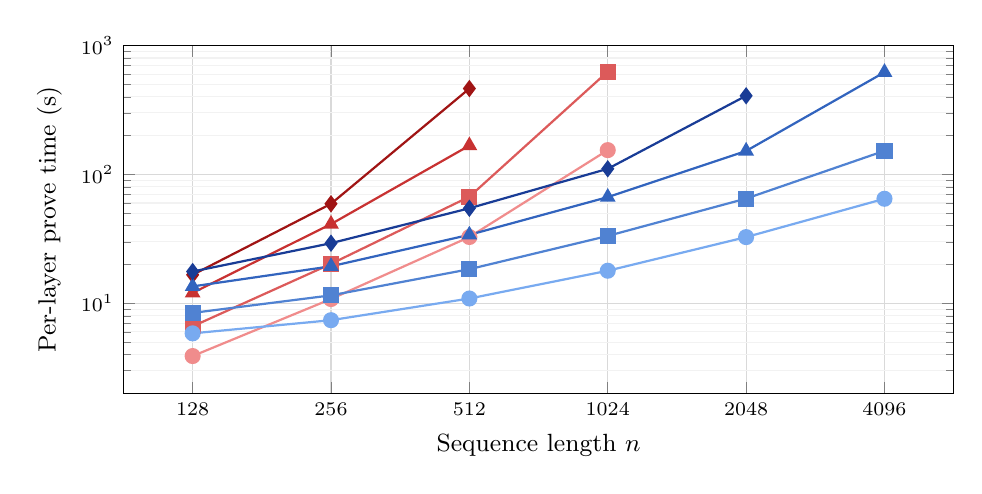
\begin{tikzpicture}
\begin{axis}[
    width=\columnwidth,
    height=6cm,
    xmode=log, ymode=log,
    log basis x=2,
    log basis y=10,
    xlabel={Sequence length $n$},
    ylabel={Per-layer prove time (s)},
    xtick={128, 256, 512, 1024, 2048, 4096},
    xticklabels={128, 256, 512, 1024, 2048, 4096},
    ymin=2, ymax=1000,
    legend to name=leg:fig6,
    legend columns=4,
    legend cell align=left,
    legend style={font=\tiny, draw=none, column sep=3pt},
    label style={font=\small},
    tick label style={font=\scriptsize},
    grid=both,
    minor grid style={gray!10},
    major grid style={gray!30},
    mark size=2.5pt,
]
% === BERT attention-only (red gradient) ===
\addplot[redspec1, mark=*, thick] coordinates {
    (128,3.90) (256,10.80) (512,32.70) (1024,154.40)
};
\addlegendentry{Tiny.Bt.}
\addplot[redspec2, mark=square*, thick] coordinates {
    (128,6.63) (256,20.23) (512,67.15) (1024,627.75)
};
\addlegendentry{Mini.Bt.}
\addplot[redspec3, mark=triangle*, thick] coordinates {
    (128,12.05) (256,41.18) (512,167.48)
};
\addlegendentry{Small.Bt.}
\addplot[redspec4, mark=diamond*, thick] coordinates {
    (128,16.65) (256,59.18) (512,463.71)
};
\addlegendentry{Base.Bt.}
% === Nystrom attention-only (blue gradient) ===
\addplot[bluespec1, mark=*, thick] coordinates {
    (128,5.85) (256,7.40) (512,10.90) (1024,17.90) (2048,32.65) (4096,64.75)
};
\addlegendentry{Tiny.Ny.}
\addplot[bluespec2, mark=square*, thick] coordinates {
    (128,8.43) (256,11.53) (512,18.40) (1024,33.33) (2048,64.98) (4096,152.43)
};
\addlegendentry{Mini.Ny.}
\addplot[bluespec3, mark=triangle*, thick] coordinates {
    (128,13.53) (256,19.38) (512,34.00) (1024,66.68) (2048,152.08) (4096,620.43)
};
\addlegendentry{Small.Ny.}
\addplot[bluespec4, mark=diamond*, thick] coordinates {
    (128,17.65) (256,29.27) (512,54.63) (1024,110.56) (2048,407.57)
};
\addlegendentry{Base.Ny.}
\end{axis}
\end{tikzpicture}\\[2pt]
\ref{leg:fig6}
\caption{Per-layer prove time for the attention equation only: BERT (red) vs.\ \nystrom (blue), log-log scale. Medium ($L{=}8$, $d{=}512$) is omitted as its per-layer cost is identical to Small ($d{=}512$).}
\label{fig:bert-vs-nystrom-freivalds}
\end{figure}

The most striking feature is the growth-rate gap: BERT's curves (red) rise steeply as $n$ increases, consistent with the $O(n^2)$ attention complexity, while \nystrom's curves (blue) grow near-linearly in the attention-only setting, reflecting $O(n)$ complexity. This translates directly into memory exhaustion: at every configuration, BERT exhausts the 128\,GB budget at a substantially shorter~$n$ than \nystrom. The feasibility gap widens as~$d$ grows: at Base ($d{=}768$, darkest shades), BERT caps at $n{=}512$ while \nystrom reaches $n{=}2048$, a $4{\times}$ extension. We omit Medium ($L{=}8$, $d{=}512$) from the figure because it yields nearly identical per-layer prove times to Small ($L{=}4$, $d{=}512$)---e.g., $167.03$\,s vs.\ $167.48$\,s for BERT at $n{=}512$---confirming the depth-invariance property: per-layer cost depends only on $d$ and $n$, not on model depth~$L$.

\sss{Quantization Fidelity}
\label{subsec:quantization-fidelity}
Table~\ref{tab:quantization} evaluates the impact of 26-bit fixed-point quantization ($k_\text{bits}{=}26$) on the pretrained uw-madison/nystromformer-512 (vocabulary size 30\,000, pretrained on BookCorpus + English Wikipedia) at sequence length $n{=}128$ over 10 batches under full cascade evaluation, where quantization errors accumulate through all 12 attention, MLP, and LayerNorm layers. The final quantized output is obtained by applying ZEN's de-quantization to the accumulated fixed-point result, and all fidelity metrics are computed on this de-quantized output. Note that the pretrained model uses $m{=}64$ landmarks (its default configuration), whereas the circuit experiments in Section~\ref{subsec:pipeline-costs} use $m{=}32$.
Top-1 agreement over all positions remains $98.8$\% and top-5 agreement is $100$\%, with cosine similarity $0.9975$. At the single \texttt{[MASK]} position the top-1 agreement drops to $90$\% but top-5 agreement stays at $100$\%, indicating that quantization primarily reshuffles near-tie predictions rather than introducing qualitatively wrong answers. These results confirm that 26-bit fixed-point arithmetic provides sufficient precision for faithful ZK-SNARK proving of transformer inference.

\begin{table}[!ht]
\centering
\caption{Quantization fidelity of 26-bit fixed-point arithmetic on a pretrained Nystr\"omformer ($d{=}768$, 12 layers, 12 heads, $m{=}64$ landmarks) at $n{=}128$.}
\label{tab:quantization}
\small
\setlength{\tabcolsep}{4pt}
\begin{tabular}{@{} ccc cc @{}}
\toprule
\multicolumn{2}{c}{Top-1 Agree.\ (\%)} & Top-5 & Cosine & RMSE \\
\cmidrule(lr){1-2}
All pos. & Mask pos. & All (\%) & Sim. & (logit) \\
\midrule
98.8 & 90.0 & 100.0 & 0.9975 & 0.378 \\
\bottomrule
\end{tabular}
\end{table}


\subsection{Conclusion and Future Work}
\label{subsec:discussion}
\sss{Practical impact} Our measurements across all five configurations (Figure~\ref{fig:bert-vs-nystrom-freivalds}) demonstrate that the combination of \nystrom low-rank attention and Freivalds randomized matrix-multiplication verification yields multiplicative constraint savings that translate directly into longer provable sequences.

\sss{Memory as the practical bottleneck} Failed runs terminate during the Groth16 trusted setup phase, which materializes the full constraint system in RAM. Peak RSS for failed runs reaches ${\sim}118$--$122$\,GB (the effective usable limit on our 128\,GB machine), confirming that setup memory---not prover computation time---is the dominant scaling bottleneck.

\sss{The MLP frontier.} While our work removes attention as the scaling bottleneck, the feed-forward MLP block emerges as the next memory frontier. We measured the cost of proving the MLP sub-circuit---identical between BERT and \nystromformer and shared by both pipelines---and report the detailed results in Appendix~\ref{appx:mlp-costs}. The measurements confirm that, once attention is optimized, the MLP becomes the dominant constraint on the maximum provable sequence length: at $d{=}512$ and above, MLP exceeds 128\,GB at all sequence lengths including $n{=}128$. Proving full-model transformer inference at sequence lengths beyond what this work demonstrates therefore requires either reducing the MLP's per-layer constraint footprint or infrastructure-level solutions such as streaming setup, distributed proving, or GPU-accelerated SNARK libraries. We view efficient ZK proving of the MLP block as a natural follow-up direction.

\sss{Per-layer cost is depth-invariant} A consistent finding across our measurements is that per-layer attention circuit cost depends only on hidden dimension~$d$ and sequence length~$n$, not on model depth~$L$. Small ($L{=}4$, $d{=}512$) and Medium ($L{=}8$, $d{=}512$) yield identical per-layer constraints, setup, and prove time; Medium's full-model costs are exactly $2{\times}$ Small's. This depth-invariance implies that our results extrapolate to deeper architectures through simple multiplication by $L$: a 24-layer model with Base-scale dimensions would require ${\sim}2{\times}$ the prove time and setup we report for $L{=}12$. The fundamental constraint is per-layer memory, not depth.

\sss{Limitations}
Our work has several limitations. \emph{(i) Single-machine CPU-only environment.} All measurements use an Apple M1 Ultra without GPU acceleration. GPU-accelerated proving or distributed proving across multiple machines would shift relative costs, particularly for larger circuits. \emph{(ii) Trusted setup.} Our Groth16-based system requires a circuit-specific trusted setup whose memory cost is our primary scaling bottleneck. Transparent SNARKs (e.g., FRI-based or IPA-based) would eliminate this at the cost of larger proof sizes and slower verification.\emph{(iii) MLP sub-circuit.} The attention sub-circuit is made tractable by our techniques, but the MLP sub-circuit remains memory-bound at $d{\geq}256$. Proving the full transformer (attention + MLP + LayerNorm) at the scales attempted here requires further techniques for the MLP block.

\begin{credits}
\subsubsection{\ackname}
To Robert, for the bagels and explaining CMYK and color spaces.

\subsubsection{\discintname}
The authors have no competing interests to declare that are relevant to the content of this article.
\end{credits}

\bibliographystyle{splncs04}
\bibliography{references}

\appendix

\section{MLP + LayerNorm Circuit Costs}
\label{appx:mlp-costs}

A complete transformer layer consists of two sub-circuits: attention and the MLP\,+\,LayerNorm block. While the main text focuses on the attention sub-circuit---the target of our zkDietFormer optimizations---we additionally measured the cost of proving the MLP\,+\,LayerNorm sub-circuit, whose constraint count is the same for BERT and \nystromformer because the MLP and LayerNorm dimensions depend only on $n$ and $d$, not on the attention mechanism.
Table~\ref{tab:mlp-costs} reports per-layer average MLP\,+\,LayerNorm costs for the Tiny configuration ($L{=}2$); all timing and memory figures are the mean of the BERT and \nystrom runs.
These measurements show that the MLP\,+\,LayerNorm sub-circuit and the attention sub-circuit contribute comparable costs at $n{=}1024$: per-layer MLP\,+\,LayerNorm proving takes $516.62$\,s versus $629.29$\,s for \nystrom-Freivalds attention. The MLP\,+\,LayerNorm block consumes $112.48$\,GB peak RAM at $n{=}1024$, making it a co-bottleneck alongside attention for memory-constrained environments.

For reference, proving a complete Tiny transformer layer (attention + MLP + LayerNorm) at $n{=}1024$ requires approximately $2{,}289.03$\,s of per-layer setup and $1{,}145.91$\,s of per-layer proving (${\sim}57$\,min total per layer). We report these measurements primarily as a baseline for future work on scalable ZK proving of the full transformer layer.

\begin{table}[H]
\centering
\caption{\textbf{MLP\,+\,LayerNorm} costs for the Tiny configuration ($L{=}2$, $d{=}128$).}
\label{tab:mlp-costs}
\resizebox{\columnwidth}{!}{%
\small
\setlength{\tabcolsep}{4pt}
\begin{tabular}{@{} l rrrrrrrr @{}}
\toprule
& & & \multicolumn{2}{c}{Commit (ms)} & & & & \\
\cmidrule(lr){4-5}
$n$ & Constr.\ (M) & Setup (s) & G16 & Lasso & Prove (s) & Verify (ms) & Proof (KB) & RAM (GB) \\
\midrule
128  & 0.98  & 94.23  & 119.3 & 147.8 & 28.38  & 285.0 & 755.8      & 26.66 \\
256  & 1.96  & 189.21 & 217.8 & 170.3 & 58.79  & 311.3 & 849.9      & 52.30 \\
512  & 3.92  & 385.63 & 441.3 & 306.0 & 137.28 & 405.5 & 1{,}026.2  & 101.93 \\
1024 & 7.84  & 883.05 & 1{,}210.3 & 433.8 & 516.62 & 482.5 & 1{,}201.7 & 112.48 \\
\bottomrule
\end{tabular}%
}
\end{table}

\section{Formal Security Definitions}
\label{appx:security-defs}

We state the formal probability conditions for the three security properties of Definition~\ref{def:zkdiet}. Notation follows Section~\ref{subsec:threat-model}.

\smallskip
\noindent\emph{Completeness.} For every $W \in \mathbb{F}^{d \times d}$ and every $\mathbf{X} \in \mathbb{F}^{n \times d}$, for $\mathsf{ck}_{\mathrm{glob}} \leftarrow \mathsf{KeyGen}(1^{\lambda}, N)$, $(\mathsf{ck}, \mathsf{pk}, \mathsf{vk}) \leftarrow \mathsf{Setup}(1^{\lambda}, \mathcal{R}_{\mathsf{zkdiet}})$, $c_{W} \leftarrow \mathsf{Commit}(\mathsf{ck}_{\mathrm{glob}}, W; o)$ and $(\mathbf{Y}', \pi) \leftarrow \mathsf{Prove}(\mathsf{pk}, \mathsf{ck}, \mathsf{ck}_{\mathrm{glob}}, \mathbf{X}; W, o)$,
\[
    \Pr\bigl[\mathsf{Verify}(\mathsf{vk}, \mathbf{X}, \mathbf{Y}', c_{W}, \pi) = 1\bigr] = 1 .
\]

\noindent\emph{Soundness.} For any PPT adversary $\mathcal{A}$, there exists a PPT extractor $\mathcal{E}$ such that
\[
  \Pr \left[
  \begin{array}{c}
    \mathsf{Verify}(\mathsf{vk}, \mathbf{X}, \mathbf{Y}^{*}, c_{W}^{*}, \pi^{*}) = 1 \\[2pt]
    \land\ \ c_{W}^{*} = \mathsf{Commit}(\mathsf{ck}_{\mathrm{glob}}, W^{*}; o^{*}) \\[2pt]
    \land\ \ \mathbf{Y}^{*} \notin \mathcal{F}^{\varepsilon}_{\mathsf{zkdiet}}(W^{*}, \mathbf{X})
  \end{array}
  \;\middle|\;
  \begin{array}{l}
    \mathsf{ck}_{\mathrm{glob}} \leftarrow \mathsf{KeyGen}(1^{\lambda}, N) \\[2pt]
    (\mathsf{ck}, \mathsf{pk}, \mathsf{vk}) \leftarrow \mathsf{Setup}(1^{\lambda}, \mathcal{R}_{\mathsf{zkdiet}}) \\[2pt]
    (c_{W}^{*}, \mathbf{X}, \mathbf{Y}^{*}, \pi^{*}) \leftarrow \mathcal{A}(\mathsf{ck}_{\mathrm{glob}}, \mathsf{ck}, \mathsf{pk}, \mathsf{vk}) \\[2pt]
    (W^{*}, o^{*}) \leftarrow \mathcal{E}^{\mathcal{A}}(\mathsf{trans}_{\mathcal{A}})
  \end{array}
  \right] \le \mathsf{negl}(\lambda).
\]

\noindent\emph{Zero-knowledge.}
Write $\mathsf{Eval}(W, \mathbf{X})$ for the deterministic off-circuit evaluation of Algorithm~3. There exists a PPT simulator $\mathcal{S} = (\mathcal{S}_{1}, \mathcal{S}_{2})$ such that for every $W$ and every PPT adversary $\mathcal{A} = (\mathcal{A}_{1}, \mathcal{A}_{2})$, the two experiments below are computationally indistinguishable (barred symbols denote simulator-produced values):
\[
\begin{array}{@{}l@{\qquad}l@{}}
\underline{\mathsf{Real}_{\mathcal{A}, W}(\lambda)} &
\underline{\mathsf{Ideal}_{\mathcal{A}, \mathcal{S}, W}(\lambda)} \\[4pt]
\mathsf{ck}_{\mathrm{glob}} \leftarrow \mathsf{KeyGen}(1^{\lambda}, N) &
(\overline{\mathsf{ck}}_{\mathrm{glob}}, \overline{\mathsf{ck}},
 \overline{\mathsf{pk}}, \overline{\mathsf{vk}}, \overline{c}_{W},
 \mathsf{td}) \leftarrow
 \mathcal{S}_{1}(1^{\lambda}, N, \mathcal{R}_{\mathsf{zkdiet}}) \\
(\mathsf{ck}, \mathsf{pk}, \mathsf{vk}) \leftarrow
 \mathsf{Setup}(1^{\lambda}, \mathcal{R}_{\mathsf{zkdiet}}) & \\
o \xleftarrow{\$} \mathcal{O};\ \
 c_{W} \leftarrow \mathsf{Commit}(\mathsf{ck}_{\mathrm{glob}}, W; o) & \\
(\mathbf{X}, st) \leftarrow \mathcal{A}_{1}(\mathsf{ck}_{\mathrm{glob}},
 \mathsf{ck}, \mathsf{pk}, \mathsf{vk}, c_{W}) &
(\mathbf{X}, st) \leftarrow
 \mathcal{A}_{1}(\overline{\mathsf{ck}}_{\mathrm{glob}},
 \overline{\mathsf{ck}}, \overline{\mathsf{pk}},
 \overline{\mathsf{vk}}, \overline{c}_{W}) \\
\mathbf{Y}' := \mathsf{Eval}(W, \mathbf{X}) &
\mathbf{Y}' := \mathsf{Eval}(W, \mathbf{X}) \\
\pi \leftarrow \mathsf{Prove}(\mathsf{pk}, \mathsf{ck},
 \mathsf{ck}_{\mathrm{glob}}, \mathbf{X}; W, o) &
\overline{\pi} \leftarrow \mathcal{S}_{2}(\mathsf{td}, \mathbf{X},
 \mathbf{Y}') \\
\mathbf{return}\ \mathcal{A}_{2}(st, \mathbf{Y}', \pi) &
\mathbf{return}\ \mathcal{A}_{2}(st, \mathbf{Y}', \overline{\pi})
\end{array}
\]
\[
\Bigl| \Pr\bigl[\mathsf{Real}_{\mathcal{A}, W}(\lambda) = 1\bigr] -
       \Pr\bigl[\mathsf{Ideal}_{\mathcal{A}, \mathcal{S}, W}(\lambda) = 1\bigr]
\Bigr| \le \mathsf{negl}(\lambda).
\]

\end{document}
